% Chapter 1

\chapter{Deep learning fundamentals} % Main chapter title
\label{Chapter2} % For referencing the chapter elsewhere, use \ref{Chapter1} 

\textbf{Summary}: \emph{This disseration makes extensive use of artificial neural networks and deep learning. In this chapter we detail the basic properties of neural networks and extend show how these ideas extend to the deep, convolutional variety of networks, key to modern image processing. We further trace the history of the development of deep learning, and its extension into the various problem domains of computer vision}

\textbf{R\'esum\'e}: \emph{Ce chapitre...}

\section{The building blocks of neural networks}
\label{sec:building_blocks_nn}

A neural network is a collection of computational units known as \emph{neurons}, organised into a sequence of \emph{layers}. An input passes \emph{forward} through a neural network, undergoing a series of transformations through combination with a set of \emph{weights} at each layer. During a training procedure, the neural network is shown examples of input data paired with target outputs. After each round of training, the neural network adjusts its (randomly initialised) weights so as to make it a little more likely to emit the target values given future appearances of the input data.

A simple neural network invokes one or more \emph{hidden layers} between input and output, for example,

\begin{align}
\mathbf{h}(\mathbf{x}) &= \sigma(\mathbf{W}^{(1)}\mathbf{x}  + \mathbf{b}^{(1)}) & \text{(hidden layer)} \notag \\
\mathbf{f}(\mathbf{x}) &= \mathcal{S}(\mathbf{W}^{(2)}\mathbf{h} + \mathbf{b}^{(2)}) & \text{(output layer)}
\end{align}

for input vector $\mathbf{x}$, first layer weights and biases matrix $\mathbf{W}^{(1)}$ and vector $\mathbf{b}^{(1)}$, and second layer weights and biases $\mathbf{W}^{(2)}$ and vector $\mathbf{b}^{(2)}$. The function $\sigma$ is a non-linear \emph{activation function}\footnote{Historically, this was the logistic function, $\sigma(x) = 1 / (1 + \exp{\{-x\}})$, a continuous approximation to the Heaviside step function (think on/off), however, in recent years, it has been superseded by the ramp function, more commonly known as the rectified linear unit, $\text{ReLU}(x) = max(0, x)$, which provides various training benefits.} and $\mathcal{S}$ is the softmax function at the output layer. The softmax is optional but often used for classification problems as it maps its inputs to categorical probabilities. In this case, the network is normally trained against a cross entropy loss function,

\begin{equation}
\mathcal{L} = \sum_i -\log(p_{y_i}),
\label{eq:neural_network_cross_entropy}
\end{equation}

where $p_{y_i} = f(\mathbf{x}_i)_{y_i}$ is the network output (probability) for the $i$th training input $\mathbf{x}_i$, indexed at the (paired) $i$th target label $y_i$ . Equation \ref{eq:neural_network_cross_entropy} is a simplification of the cross entropy formula for the case where the $y_i$ are ``one-hot'' vectors. Note that neural networks can be trained for classification, regression, or unsupervised feature extraction, depending on the requirements of the data. Each entails a different output layer and loss function for the network. Figure \ref{fig:neural_network} depicts an examle of our simple neural network \emph{architecture}.

\begin{figure}
\centering


\tikzset{every picture/.style={line width=0.75pt}} %set default line width to 0.75pt        

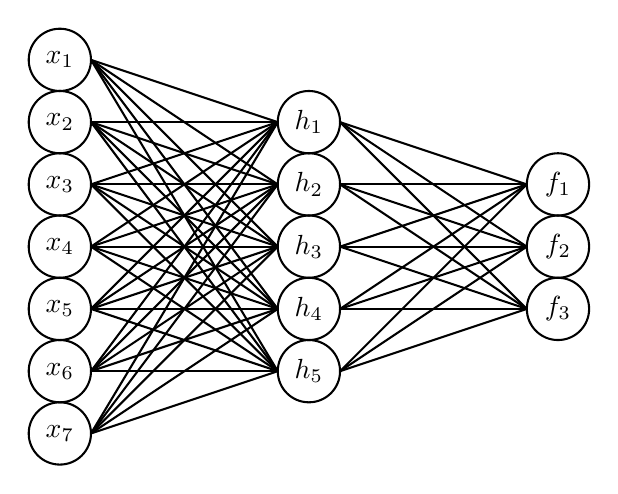
\begin{tikzpicture}[x=0.75pt,y=0.75pt,yscale=-1,xscale=1]
%uncomment if require: \path (0,280); %set diagram left start at 0, and has height of 280

%Shape: Circle [id:dp6274252196607965] 
\draw   (0,46) .. controls (0,37.72) and (6.72,31) .. (15,31) .. controls (23.28,31) and (30,37.72) .. (30,46) .. controls (30,54.28) and (23.28,61) .. (15,61) .. controls (6.72,61) and (0,54.28) .. (0,46) -- cycle ;
%Shape: Circle [id:dp5375048559550425] 
\draw   (0,76) .. controls (0,67.72) and (6.72,61) .. (15,61) .. controls (23.28,61) and (30,67.72) .. (30,76) .. controls (30,84.28) and (23.28,91) .. (15,91) .. controls (6.72,91) and (0,84.28) .. (0,76) -- cycle ;
%Shape: Circle [id:dp1827624457133501] 
\draw   (0,166) .. controls (0,157.72) and (6.72,151) .. (15,151) .. controls (23.28,151) and (30,157.72) .. (30,166) .. controls (30,174.28) and (23.28,181) .. (15,181) .. controls (6.72,181) and (0,174.28) .. (0,166) -- cycle ;
%Shape: Circle [id:dp86041947411614] 
\draw   (0,106) .. controls (0,97.72) and (6.72,91) .. (15,91) .. controls (23.28,91) and (30,97.72) .. (30,106) .. controls (30,114.28) and (23.28,121) .. (15,121) .. controls (6.72,121) and (0,114.28) .. (0,106) -- cycle ;
%Shape: Circle [id:dp705040127477171] 
\draw   (0,136) .. controls (0,127.72) and (6.72,121) .. (15,121) .. controls (23.28,121) and (30,127.72) .. (30,136) .. controls (30,144.28) and (23.28,151) .. (15,151) .. controls (6.72,151) and (0,144.28) .. (0,136) -- cycle ;
%Shape: Circle [id:dp5072233804745877] 
\draw   (0,196) .. controls (0,187.72) and (6.72,181) .. (15,181) .. controls (23.28,181) and (30,187.72) .. (30,196) .. controls (30,204.28) and (23.28,211) .. (15,211) .. controls (6.72,211) and (0,204.28) .. (0,196) -- cycle ;
%Shape: Circle [id:dp8596927023792] 
\draw   (0,16) .. controls (0,7.72) and (6.72,1) .. (15,1) .. controls (23.28,1) and (30,7.72) .. (30,16) .. controls (30,24.28) and (23.28,31) .. (15,31) .. controls (6.72,31) and (0,24.28) .. (0,16) -- cycle ;
%Shape: Circle [id:dp7075342175624237] 
\draw   (240,76) .. controls (240,67.72) and (246.72,61) .. (255,61) .. controls (263.28,61) and (270,67.72) .. (270,76) .. controls (270,84.28) and (263.28,91) .. (255,91) .. controls (246.72,91) and (240,84.28) .. (240,76) -- cycle ;
%Shape: Circle [id:dp8919445675047236] 
\draw   (240,106) .. controls (240,97.72) and (246.72,91) .. (255,91) .. controls (263.28,91) and (270,97.72) .. (270,106) .. controls (270,114.28) and (263.28,121) .. (255,121) .. controls (246.72,121) and (240,114.28) .. (240,106) -- cycle ;
%Shape: Circle [id:dp5251355385061629] 
\draw   (240,136) .. controls (240,127.72) and (246.72,121) .. (255,121) .. controls (263.28,121) and (270,127.72) .. (270,136) .. controls (270,144.28) and (263.28,151) .. (255,151) .. controls (246.72,151) and (240,144.28) .. (240,136) -- cycle ;
%Straight Lines [id:da9408609688043365] 
\draw    (30,16) -- (120,46) ;
%Straight Lines [id:da8004597444193696] 
\draw    (30,46) -- (120,46) ;
%Straight Lines [id:da8964766936449153] 
\draw    (30,76) -- (120,46) ;
%Straight Lines [id:da18932408343565388] 
\draw    (30,106) -- (120,46) ;
%Straight Lines [id:da058680739240724256] 
\draw    (30,136) -- (120,46) ;
%Straight Lines [id:da9046089810150858] 
\draw    (30,166) -- (120,46) ;
%Straight Lines [id:da5082059060971128] 
\draw    (30,196) -- (120,46) ;
%Straight Lines [id:da9256273161065741] 
\draw    (30,46) -- (120,76) ;
%Straight Lines [id:da2602977405689222] 
\draw    (30,76) -- (120,76) ;
%Straight Lines [id:da12125091141593869] 
\draw    (30,106) -- (120,76) ;
%Straight Lines [id:da08135123675872669] 
\draw    (30,136) -- (120,76) ;
%Straight Lines [id:da5858631998790831] 
\draw    (30,166) -- (120,76) ;
%Straight Lines [id:da17596157294922132] 
\draw    (30,196) -- (120,76) ;
%Straight Lines [id:da9925378930893565] 
\draw    (30,76) -- (120,106) ;
%Straight Lines [id:da5207395174325888] 
\draw    (30,106) -- (120,106) ;
%Straight Lines [id:da8248512549102488] 
\draw    (30,136) -- (120,106) ;
%Straight Lines [id:da3519507316262549] 
\draw    (30,166) -- (120,106) ;
%Straight Lines [id:da6640848412724859] 
\draw    (30,196) -- (120,106) ;
%Straight Lines [id:da997942803644863] 
\draw    (30,106) -- (120,136) ;
%Straight Lines [id:da7487557927165537] 
\draw    (30,136) -- (120,136) ;
%Straight Lines [id:da7611944271887731] 
\draw    (30,166) -- (120,136) ;
%Straight Lines [id:da21301748797978537] 
\draw    (30,196) -- (120,136) ;
%Straight Lines [id:da3139323398801428] 
\draw    (30,136) -- (120,166) ;
%Straight Lines [id:da20938664574220855] 
\draw    (30,166) -- (120,166) ;
%Straight Lines [id:da6184238449229069] 
\draw    (30,196) -- (120,166) ;
%Straight Lines [id:da3083040605561572] 
\draw    (30,106) -- (120,166) ;
%Straight Lines [id:da45278089591104165] 
\draw    (30,76) -- (120,136) ;
%Straight Lines [id:da24381797487662027] 
\draw    (30,76) -- (120,166) ;
%Straight Lines [id:da48942345034602286] 
\draw    (30,46) -- (120,166) ;
%Straight Lines [id:da29330955425665184] 
\draw    (30,46) -- (120,136) ;
%Straight Lines [id:da9820116600675901] 
\draw    (30,46) -- (120,106) ;
%Straight Lines [id:da4074766428865084] 
\draw    (30,16) -- (120,76) ;
%Straight Lines [id:da5228559700478754] 
\draw    (30,16) -- (120,106) ;
%Straight Lines [id:da7147227122291991] 
\draw    (30,16) -- (120,136) ;
%Straight Lines [id:da6097206892931846] 
\draw    (30,16) -- (120,166) ;
%Shape: Circle [id:dp11242648757557339] 
\draw   (120,46) .. controls (120,37.72) and (126.72,31) .. (135,31) .. controls (143.28,31) and (150,37.72) .. (150,46) .. controls (150,54.28) and (143.28,61) .. (135,61) .. controls (126.72,61) and (120,54.28) .. (120,46) -- cycle ;
%Shape: Circle [id:dp9050841701170105] 
\draw   (120,76) .. controls (120,67.72) and (126.72,61) .. (135,61) .. controls (143.28,61) and (150,67.72) .. (150,76) .. controls (150,84.28) and (143.28,91) .. (135,91) .. controls (126.72,91) and (120,84.28) .. (120,76) -- cycle ;
%Shape: Circle [id:dp5041080162745605] 
\draw   (120,166) .. controls (120,157.72) and (126.72,151) .. (135,151) .. controls (143.28,151) and (150,157.72) .. (150,166) .. controls (150,174.28) and (143.28,181) .. (135,181) .. controls (126.72,181) and (120,174.28) .. (120,166) -- cycle ;
%Shape: Circle [id:dp29510144828888285] 
\draw   (120,106) .. controls (120,97.72) and (126.72,91) .. (135,91) .. controls (143.28,91) and (150,97.72) .. (150,106) .. controls (150,114.28) and (143.28,121) .. (135,121) .. controls (126.72,121) and (120,114.28) .. (120,106) -- cycle ;
%Shape: Circle [id:dp38568855968083915] 
\draw   (120,136) .. controls (120,127.72) and (126.72,121) .. (135,121) .. controls (143.28,121) and (150,127.72) .. (150,136) .. controls (150,144.28) and (143.28,151) .. (135,151) .. controls (126.72,151) and (120,144.28) .. (120,136) -- cycle ;
%Straight Lines [id:da5360486561481052] 
\draw    (150,46) -- (240,76) ;
%Straight Lines [id:da19202323798355136] 
\draw    (150,76) -- (240,76) ;
%Straight Lines [id:da7401225576679021] 
\draw    (150,106) -- (240,76) ;
%Straight Lines [id:da344828522461311] 
\draw    (150,136) -- (240,76) ;
%Straight Lines [id:da6037747089314498] 
\draw    (150,166) -- (240,76) ;
%Straight Lines [id:da04320697434128862] 
\draw    (150,76) -- (240,106) ;
%Straight Lines [id:da8253115326188497] 
\draw    (150,106) -- (240,106) ;
%Straight Lines [id:da8994788857674927] 
\draw    (150,136) -- (240,106) ;
%Straight Lines [id:da15316881383985992] 
\draw    (150,166) -- (240,106) ;
%Straight Lines [id:da7634695012747197] 
\draw    (150,106) -- (240,136) ;
%Straight Lines [id:da8030324872099031] 
\draw    (150,136) -- (240,136) ;
%Straight Lines [id:da6478174350864642] 
\draw    (150,166) -- (240,136) ;
%Straight Lines [id:da14147982747602306] 
\draw    (150,76) -- (240,136) ;
%Straight Lines [id:da12312326634465576] 
\draw    (150,46) -- (240,136) ;
%Straight Lines [id:da3359788891048011] 
\draw    (150,46) -- (240,106) ;

% % Text Node
% \draw (13,225) node    {$\mathbf{x}$};
% % Text Node
% \draw (133.5,234.5) node    {$\underbrace{\sigma \left( W^{( 1)}\mathbf{x} +b^{( 1)}\right)}_{\mathbf{h}(\mathbf{x}\}}$};
% % Text Node
% \draw (253,221.5) node    {$\mathcal{S}\left( W^{( 2)}\mathbf{h} +b^{( 2)}\right)$};
% Text Node
\draw (15,16) node    {$x_{1}$};
% Text Node
\draw (15,46) node    {$x_{2}$};
% Text Node
\draw (15,76) node    {$x_{3}$};
% Text Node
\draw (15,106) node    {$x_{4}$};
% Text Node
\draw (15,136) node    {$x_{5}$};
% Text Node
\draw (15,166) node    {$x_{6}$};
% Text Node
\draw (15,196) node    {$x_{7}$};
% Text Node
\draw (135,46) node    {$h_{1}$};
% Text Node
\draw (135,76) node    {$h_{2}$};
% Text Node
\draw (135,106) node    {$h_{3}$};
% Text Node
\draw (135,136) node    {$h_{4}$};
% Text Node
\draw (135,166) node    {$h_{5}$};
% Text Node
\draw (255,76) node    {$f_{1}$};
% Text Node
\draw (255,106) node    {$f_{2}$};
% Text Node
\draw (255,136) node    {$f_{3}$};
\end{tikzpicture}

\caption{Fully-connected neural network with $7$ input neurons, a single hidden layer with $5$ neurons, and an output layer with $3$ neurons.}
\label{fig:neural_network}
\end{figure}

The neural network framework gives us freedom over the number of layers and the number of neurons in each layer. The more neurons, the more expressive the network, yet the more likely overfitting becomes\footnote{It is rare to require more than three layers, however, and exceeding this amount will be done to exploit deep hierarchical structures in the data.}. We may extend to a multi-layer network simply by stacking the desired number of layers,

\begin{equation}
\mathbf{f}(\mathbf{x}) = \mathcal{S}(\mathbf{W}^{(M)}\sigma(\mathbf{W}^{(M-1)}(\cdots\sigma(\mathbf{W}^{(1)}\mathbf{x} + \mathbf{b}^{(1)})\cdots) + \mathbf{b}^{(M-1)})  + \mathbf{b}^{(M)})
\end{equation}

Thus, the network layers are linear transformations interspersed with non-linear functions. When the inputs correlate positively with a vector of weights, the corresponding hidden layer neuron tends to become active via the non-linearity. In this way, each neuron of a hidden layer amounts to a feature detector for the prior layer. The hidden layer activations are then recombined in the next layer, and so on, allowing for ever more complex aggregations of features. This is the essence of deep learning. However, this tends not to work very well without certain inductive biases, (and, indeed, an amenable dataset) which we will encounter in Section \ref{sec:convolutional_neural_networks}. Despite their inherent non-linearity, and non-convexity, neural networks can be trained with standard gradient descent,

\begin{equation}
\theta_{t+1} \leftarrow \theta_t - \alpha \cdot \nabla_{\theta}\mathcal{L}
\label{eq:gradient_descent}
\end{equation}

for the full set of model parameters $\theta$ and \emph{learning rate} $\alpha$. More sophisticated update rules than vanilla gradient descent exist such as RMSprop (\cite{tieleman2012lecture}), and Adam (\cite{kingma2014adam}). These methods improve over the Equation \ref{eq:gradient_descent} by adapting a learning rate for each parameter (rather than one-size-fits-all). Whatever the chosen method, the gradients are always computed using the backpropagation algorithm, which we describe presently.

%\begin{figure}
%\centering
%\begin{tabular}{cc}
%\subfloat[]{\includegraphics[width=0.49\textwidth]{Figures/universalapproximater.pdf}} & 
%\subfloat[]{\includegraphics[width=0.5\textwidth]{Figures/sgd.pdf}}
% \end{tabular}
% \caption{A simple example of a neural network fitting an absolute value function (A) and the corresponding learning curve for stochastic gradient descent (B). Generated with \texttt{mlpDemo.m}.}
% \label{fig:universalapproximater}
% \end{figure}

\subsection{Backpropagation}

The procedure for computing the gradients at each iteration of gradient descent is called backpropagation. Backpropagation is an application of the chain rule to the graphical structure of the neural network. The crucial formula for backpropagation, as presented in \cite{rumelhart1985learning} is,

\begin{equation}
\frac{\partial L}{\partial x_i} = \sum_j \frac{\partial L}{\partial y_{ij}}\cdot\frac{\partial y_{ij}}{\partial x_i},
\label{eq:backpropagation}
\end{equation}

that is, the gradient of neuron $x_i$ at a given layer $l$ is the sum product of the gradients of the neurons emanating from it $y_{ij}$ and the gradient of the connection between them. From a practical standpoint, each layer $l$ over which we perform backpropagation requires three computations:

\begin{enumerate}
\item $\frac{\partial L}{\partial \mathbf{s}^{(l)}}$, the gradient of the \emph{scores}, $\mathbf{s}^{(l)} = \mathbf{W}^{(l)}\mathbf{x}^{(l)} + \mathbf{b}^{(l)}$. Note this is a ``pseudo-layer'' between the linear transformation and the activation.
\item $\frac{\partial L}{\partial \mathbf{W}^{(l)}}$, the gradient of the weights. These are recorded to ultimately make the descent step (Equation \ref{eq:gradient_descent}).
\item $\frac{\partial L}{\partial \mathbf{x}^{(l)}} = \frac{\partial L}{\partial \mathbf{\sigma}^{(l-1)}}$, the gradient of the input (previous activation). This is the \emph{error signal} that is passed back to the layer below.
\end{enumerate}

Let us first consider (1), the gradient of the scores. In general, we compute, $\frac{\partial L}{\partial \mathbf{s}^{(l)}} = \frac{\partial L}{\partial \boldsymbol\sigma^{(l)}}\cdot\frac{\partial\boldsymbol\sigma^{(l)}}{\partial\mathbf{s}^{(l)}}$ where $\frac{\partial L}{\partial \boldsymbol\sigma^{(l)}} = \frac{\partial L}{\partial \mathbf{x}^{(l+1)}}$, since the activation of the present layer is the input to the following layer. The activation function $\sigma$ is applied element-wise. Consequently, in the pseudo-layer between linear transform and activation, each neuron has a single connection. Therefore, with respect to Equation \ref{eq:backpropagation}, the sum reduces to a single element per gradient giving,

% Since we have $\sigma(\mathbf{s}) = [\sigma(s_1), \sigma(s_2), \cdots \sigma(s_k)]^T$, an element-wise transformation, we can calculate the gradient element-wise as,

\begin{equation}
\frac{\partial L}{\partial \mathbf{s}^{(l)}} =
\begin{bmatrix}
\frac{\partial L}{\partial\sigma_1^{(l)}}\cdot\frac{\partial\sigma_1^{(l)}}{\partial{s}_1^{(l)}} \\ 
\vdots \\
\frac{\partial L}{\partial\sigma_k^{(l)}}\cdot\frac{\partial\sigma_k^{(l)}}{\partial{s}_k^{(l)}} \\
\end{bmatrix},
\label{eq:backprop_scores}
\end{equation}

where for sigmoid, $\frac{\partial\sigma_i^{(l)}}{\partial{s}_i^{(l)}} = \partial\sigma_i^{(l)}(1 - \sigma_i^{(l)})$, and for ReLU, $\frac{\partial\sigma_i^{(l)}}{\partial{s}_i^{(l)}} = 1_{\{\sigma_i^{(l)} > 0\}}$.

For computation (2), the weights gradient, consider, $\frac{\partial L}{\partial w_{kj}^{(l)}} = \frac{\partial L}{\partial s_j}\cdot\frac{\partial s_j}{\partial w_{kj}^{(l)}} = \frac{\partial L}{\partial s_j}\cdot x_j$. In vector form this gives us, $\frac{\partial L}{\partial \mathbf{s}^{(l)}}\mathbf{x}^T$, that is, the outer product of the score gradient and the input vector. Considering that the loss over a batch is the sum of losses for each sample, we have in general, for batch $\mathbf{X} \in \mathbb{R}^{D \times M}$,

\begin{equation}
\frac{\partial L}{\partial \mathbf{W}^{(l)}} = \frac{\partial L}{\partial \mathbf{s}^{(l)}}\cdot\mathbf{X}^T
\label{eq:backprop_weights}
\end{equation}

For the bias terms, consider that with the bias trick, the gradients $\frac{\partial s_j}{\partial b_{k}^{(l)}} = 1, \forall k$. We can therefore simply sum the score gradients over the size $m$ batch, $\sum_m\frac{\partial s_{mj}}{\partial b_{k}^{(l)}}$. 

Finally, for computation (3), simply consider the chain rule, $\frac{\partial L}{\partial\mathbf{x}^{(l)}} = \frac{\partial L}{\partial\mathbf{s}^{(l)}}\cdot\frac{\partial\mathbf{s}^{(l)}}{\partial\mathbf{x}^{(l)}}.$ It is easy to show by forming the Jacobian matrix that $\frac{\partial\mathbf{s}^{(l)}}{\partial\mathbf{x}^{(l)}} = \mathbf{W}^{(l)}$. Hence,

\begin{equation}
\frac{\partial L}{\partial \mathbf{x}^{(l)}} = \frac{\partial L}{\partial \mathbf{s}^{(l)}}\cdot\mathbf{W}^T
\label{eq:backprop_activations}
\end{equation}

This final gradient is passed to the previous layer as $\frac{\partial L}{\partial \boldsymbol{\sigma}^{(l-1)}}$ to continue the backpropagation. Upon traversing the network layers, the weight gradients are used to update to weights as in Equation \ref{eq:gradient_descent}.

\section{Convolutional neural networks}
\label{sec:convolutional_neural_networks}

\begin{figure}[h]
\centering


\tikzset{every picture/.style={line width=0.75pt}} %set default line width to 0.75pt        

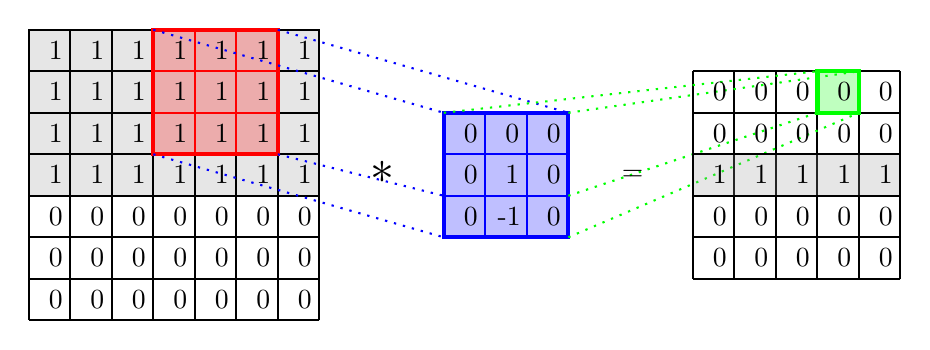
\begin{tikzpicture}[x=0.75pt,y=0.75pt,yscale=-1,xscale=1]
%uncomment if require: \path (0,300); %set diagram left start at 0, and has height of 300

%Shape: Rectangle [id:dp25487360212559773] 
\draw  [fill={rgb, 255:red, 155; green, 155; blue, 155 }  ,fill opacity=0.25 ] (20,40) -- (160,40) -- (160,120) -- (20,120) -- cycle ;
%Straight Lines [id:da48070318806651446] 
\draw [color={rgb, 255:red, 0; green, 0; blue, 255 }  ,draw opacity=1 ]   (240,80) -- (240,140) ;
%Straight Lines [id:da4220387714515078] 
\draw [color={rgb, 255:red, 0; green, 0; blue, 255 }  ,draw opacity=1 ]   (260,80) -- (260,140) ;
%Straight Lines [id:da7320635562801635] 
\draw [color={rgb, 255:red, 0; green, 0; blue, 255 }  ,draw opacity=1 ]   (280,100) -- (220,100) ;
%Straight Lines [id:da5517409302166617] 
\draw [color={rgb, 255:red, 0; green, 0; blue, 255 }  ,draw opacity=1 ]   (280,120) -- (220,120) ;
%Straight Lines [id:da49426492926027354] 
\draw    (40,40) -- (40,100) ;
%Straight Lines [id:da23292785234016555] 
\draw    (60,40) -- (60,100) ;
%Straight Lines [id:da651404528538615] 
\draw    (80,60) -- (20,60) ;
%Straight Lines [id:da4843799878266911] 
\draw    (80,80) -- (20,80) ;
%Straight Lines [id:da6254275230076098] 
\draw    (80,100) -- (20,100) ;
%Straight Lines [id:da4233740356676763] 
\draw [color={rgb, 255:red, 255; green, 0; blue, 0 }  ,draw opacity=1 ]   (100,40) -- (100,100) ;
%Straight Lines [id:da5341280803827987] 
\draw [color={rgb, 255:red, 255; green, 0; blue, 0 }  ,draw opacity=1 ]   (120,40) -- (120,100) ;
%Straight Lines [id:da13302075277978864] 
\draw [color={rgb, 255:red, 255; green, 0; blue, 0 }  ,draw opacity=1 ]   (140,60) -- (80,60) ;
%Straight Lines [id:da9863194899022711] 
\draw [color={rgb, 255:red, 255; green, 0; blue, 0 }  ,draw opacity=1 ]   (140,80) -- (80,80) ;
%Straight Lines [id:da7662744945480855] 
\draw    (20,120) -- (20,180) ;
%Straight Lines [id:da9543501657360597] 
\draw    (40,100) -- (40,180) ;
%Straight Lines [id:da11307759095344994] 
\draw    (60,100) -- (60,180) ;
%Straight Lines [id:da8456940945284525] 
\draw    (80,100) -- (80,180) ;
%Straight Lines [id:da8499806788240366] 
\draw    (80,140) -- (20,140) ;
%Straight Lines [id:da7280775347460067] 
\draw    (80,160) -- (20,160) ;
%Straight Lines [id:da601676691043139] 
\draw    (100,100) -- (100,180) ;
%Straight Lines [id:da5376052265939861] 
\draw    (120,100) -- (120,180) ;
%Straight Lines [id:da8420085026713285] 
\draw    (140,100) -- (140,180) ;
%Straight Lines [id:da8602642598665121] 
\draw    (160,140) -- (80,140) ;
%Straight Lines [id:da34376125037992533] 
\draw    (160,160) -- (80,160) ;
%Straight Lines [id:da4190745792908639] 
\draw    (160,120) -- (160,180) ;
%Straight Lines [id:da47552153609272807] 
\draw    (160,180) -- (20,180) ;
%Straight Lines [id:da5153224088417779] 
\draw    (360,60) -- (360,80) ;
%Straight Lines [id:da3474912223128712] 
\draw    (360,80) -- (340,80) ;
%Straight Lines [id:da5029916779965798] 
\draw    (380,60) -- (380,80) ;
%Straight Lines [id:da5570584559169737] 
\draw    (400,80) -- (360,80) ;
%Straight Lines [id:da9162604250778118] 
\draw    (360,80) -- (360,160) ;
%Straight Lines [id:da40719365471832236] 
\draw    (360,100) -- (340,100) ;
%Straight Lines [id:da034362844862375064] 
\draw    (360,120) -- (340,120) ;
%Straight Lines [id:da685438913141074] 
\draw    (360,140) -- (340,140) ;
%Straight Lines [id:da8424205523711409] 
\draw    (380,80) -- (380,160) ;
%Straight Lines [id:da8858347221436383] 
\draw    (400,80) -- (400,160) ;
%Straight Lines [id:da27029739217568005] 
\draw    (420,80) -- (420,160) ;
%Straight Lines [id:da6291825687218066] 
\draw    (440,100) -- (360,100) ;
%Straight Lines [id:da24616407324119416] 
\draw    (440,120) -- (360,120) ;
%Straight Lines [id:da6953566761731363] 
\draw    (440,140) -- (360,140) ;
%Straight Lines [id:da41781897975044424] 
\draw    (440,60) -- (440,160) ;
%Straight Lines [id:da9024504416708067] 
\draw    (440,160) -- (340,160) ;
%Straight Lines [id:da437487469113194] 
\draw    (340,160) -- (340,60) ;
%Straight Lines [id:da42856804153576733] 
\draw    (340,60) -- (400,60) ;
%Straight Lines [id:da29742318731815276] 
\draw    (160,100) -- (140,100) ;
%Straight Lines [id:da6342806628866308] 
\draw    (160,80) -- (140,80) ;
%Straight Lines [id:da8322538094905481] 
\draw    (160,60) -- (140,60) ;
%Straight Lines [id:da4771522388518019] 
\draw    (440,80) -- (420,80) ;
%Straight Lines [id:da6252610685871461] 
\draw    (440,60) -- (420,60) ;
%Shape: Square [id:dp7520015492630954] 
\draw  [color={rgb, 255:red, 255; green, 0; blue, 0 }  ,draw opacity=1 ][fill={rgb, 255:red, 255; green, 0; blue, 0 }  ,fill opacity=0.25 ][line width=1.5]  (80,40) -- (140,40) -- (140,100) -- (80,100) -- cycle ;
%Shape: Square [id:dp34706602029160105] 
\draw  [color={rgb, 255:red, 0; green, 0; blue, 255 }  ,draw opacity=1 ][fill={rgb, 255:red, 0; green, 0; blue, 255 }  ,fill opacity=0.25 ][line width=1.5]  (220,80) -- (280,80) -- (280,140) -- (220,140) -- cycle ;
%Shape: Square [id:dp31945592977082327] 
\draw  [color={rgb, 255:red, 0; green, 255; blue, 0 }  ,draw opacity=1 ][fill={rgb, 255:red, 0; green, 255; blue, 0 }  ,fill opacity=0.25 ][line width=1.5]  (400,60) -- (420,60) -- (420,80) -- (400,80) -- cycle ;
%Straight Lines [id:da4076888961238452] 
\draw [color={rgb, 255:red, 0; green, 0; blue, 255 }  ,draw opacity=1 ][line width=0.75]  [dash pattern={on 0.84pt off 2.51pt}]  (80,40) -- (220,80) ;
%Straight Lines [id:da4927704574255918] 
\draw [color={rgb, 255:red, 0; green, 0; blue, 255 }  ,draw opacity=1 ][line width=0.75]  [dash pattern={on 0.84pt off 2.51pt}]  (140,40) -- (280,80) ;
%Straight Lines [id:da40688229012518395] 
\draw [color={rgb, 255:red, 0; green, 0; blue, 255 }  ,draw opacity=1 ][line width=0.75]  [dash pattern={on 0.84pt off 2.51pt}]  (80,100) -- (220,140) ;
%Straight Lines [id:da8353046610007115] 
\draw [color={rgb, 255:red, 0; green, 0; blue, 255 }  ,draw opacity=1 ][line width=0.75]  [dash pattern={on 0.84pt off 2.51pt}]  (140,100) -- (220,120) ;
%Straight Lines [id:da5435823681859943] 
\draw [color={rgb, 255:red, 0; green, 255; blue, 0 }  ,draw opacity=1 ][line width=0.75]  [dash pattern={on 0.84pt off 2.51pt}]  (220,80) -- (400,60) ;
%Straight Lines [id:da24116800664031957] 
\draw [color={rgb, 255:red, 0; green, 255; blue, 0 }  ,draw opacity=1 ][line width=0.75]  [dash pattern={on 0.84pt off 2.51pt}]  (280,80) -- (420,60) ;
%Straight Lines [id:da44351434305101745] 
\draw [color={rgb, 255:red, 0; green, 255; blue, 0 }  ,draw opacity=1 ][line width=0.75]  [dash pattern={on 0.84pt off 2.51pt}]  (280,120) -- (400,80) ;
%Straight Lines [id:da5637906228581073] 
\draw [color={rgb, 255:red, 0; green, 255; blue, 0 }  ,draw opacity=1 ][line width=0.75]  [dash pattern={on 0.84pt off 2.51pt}]  (280,140) -- (420,80) ;
%Shape: Rectangle [id:dp8345669388194714] 
\draw  [fill={rgb, 255:red, 155; green, 155; blue, 155 }  ,fill opacity=0.25 ] (340,100) -- (440,100) -- (440,120) -- (340,120) -- cycle ;

% Text Node
\draw (190.5,108.5) node  [font=\LARGE] [align=left] {$\displaystyle *$};
% Text Node
\draw (311,110) node    {$=$};
% Text Node
\draw (93,50) node    {$1$};
% Text Node
\draw (113,50) node    {$1$};
% Text Node
\draw (133,50) node    {$1$};
% Text Node
\draw (93,70) node    {$1$};
% Text Node
\draw (113,70) node    {$1$};
% Text Node
\draw (133,70) node    {$1$};
% Text Node
\draw (93,90) node    {$1$};
% Text Node
\draw (113,90) node    {$1$};
% Text Node
\draw (133,90) node    {$1$};
% Text Node
\draw (233,90) node    {$0$};
% Text Node
\draw (253,90) node    {$0$};
% Text Node
\draw (273,90) node    {$0$};
% Text Node
\draw (233,110) node    {$0$};
% Text Node
\draw (233,130) node    {$0$};
% Text Node
\draw (251.5,130) node    {-$1$};
% Text Node
\draw (273,130) node    {$0$};
% Text Node
\draw (273,110) node    {$0$};
% Text Node
\draw (253,110) node    {$1$};
% Text Node
\draw (33,50) node    {$1$};
% Text Node
\draw (53,50) node    {$1$};
% Text Node
\draw (53,70) node    {$1$};
% Text Node
\draw (53,90) node    {$1$};
% Text Node
\draw (73,50) node    {$1$};
% Text Node
\draw (73,70) node    {$1$};
% Text Node
\draw (33,70) node    {$1$};
% Text Node
\draw (33,90) node    {$1$};
% Text Node
\draw (53,110) node    {$1$};
% Text Node
\draw (73,130) node    {$0$};
% Text Node
\draw (93,150) node    {$0$};
% Text Node
\draw (113,170) node    {$0$};
% Text Node
\draw (73,110) node    {$1$};
% Text Node
\draw (93,130) node    {$0$};
% Text Node
\draw (113,150) node    {$0$};
% Text Node
\draw (133,170) node    {$0$};
% Text Node
\draw (73,90) node    {$1$};
% Text Node
\draw (93,110) node    {$1$};
% Text Node
\draw (113,130) node    {$0$};
% Text Node
\draw (133,150) node    {$0$};
% Text Node
\draw (153,170) node    {$0$};
% Text Node
\draw (113,110) node    {$1$};
% Text Node
\draw (133,130) node    {$0$};
% Text Node
\draw (153,150) node    {$0$};
% Text Node
\draw (133,110) node    {$1$};
% Text Node
\draw (153,130) node    {$0$};
% Text Node
\draw (153,110) node    {$1$};
% Text Node
\draw (153,90) node    {$1$};
% Text Node
\draw (153,70) node    {$1$};
% Text Node
\draw (153,50) node    {$1$};
% Text Node
\draw (33,110) node    {$1$};
% Text Node
\draw (53,130) node    {$0$};
% Text Node
\draw (73,150) node    {$0$};
% Text Node
\draw (93,170) node    {$0$};
% Text Node
\draw (33,130) node    {$0$};
% Text Node
\draw (53,150) node    {$0$};
% Text Node
\draw (73,170) node    {$0$};
% Text Node
\draw (33,150) node    {$0$};
% Text Node
\draw (53,170) node    {$0$};
% Text Node
\draw (33,170) node    {$0$};
% Text Node
\draw (353,70) node    {$0$};
% Text Node
\draw (373,90) node    {$0$};
% Text Node
\draw (393,110) node    {$1$};
% Text Node
\draw (413,130) node    {$0$};
% Text Node
\draw (433,150) node    {$0$};
% Text Node
\draw (373,70) node    {$0$};
% Text Node
\draw (393,90) node    {$0$};
% Text Node
\draw (413,110) node    {$1$};
% Text Node
\draw (433,130) node    {$0$};
% Text Node
\draw (353,90) node    {$0$};
% Text Node
\draw (373,110) node    {$1$};
% Text Node
\draw (393,130) node    {$0$};
% Text Node
\draw (413,150) node    {$0$};
% Text Node
\draw (393,70) node    {$0$};
% Text Node
\draw (413,90) node    {$0$};
% Text Node
\draw (433,110) node    {$1$};
% Text Node
\draw (433,70) node    {$0$};
% Text Node
\draw (433,90) node    {$0$};
% Text Node
\draw (393,150) node    {$0$};
% Text Node
\draw (373,130) node    {$0$};
% Text Node
\draw (373,150) node    {$0$};
% Text Node
\draw (353,150) node    {$0$};
% Text Node
\draw (353,130) node    {$0$};
% Text Node
\draw (353,110) node    {$1$};
% Text Node
\draw (413,70) node    {$0$};


\end{tikzpicture}


\caption{Convolution operation consisting of (from left to right) an input image, convolutional kernel, and convolved output image. The \emph{valid} convolution results in the loss of the border pixels. Notice how the output represents the gradient image, obtained by setting the kernel to the finite difference between vertically adjacent pixels.}
\label{fig:convolution_operation}
\end{figure}

Convolutional neural networks (CNNs) are a family of neural network architectures having at least one \emph{convolutional layer}. In image processing, a convolution between an image $\mathbf{I}$ and \emph{kernel} $\mathbf{K}$ of size $d \times d$ and centered at a given pixel $(x, y)$ is defined as,

\begin{equation}
(\mathbf{I} * \mathbf{K})(x, y) = \sum_{i = 1}^{d}\sum_{j = 1}^{d} \mathbf{I}(x + i -d/2, y + j - d/2) \times \mathbf{K}(i, j),
\label{eq:convolution_operation}
\end{equation}

and is illustrated in Figure \ref{fig:convolution_operation}. Convolutions are useful for operations such as feature extraction and edge detection. A CNN is a neural network explicitly wired to perform convolutions\footnote{A convolutional layer can still be represented as a sparse fully-connected layer.}. In a convolutional layer, the elements of kernel $\mathbf{K}$ become learnable weights, replacing the large, fully-connected weight matrices from Section \ref{sec:building_blocks_nn}. In effect, the weights are \emph{shared} across the input surface, greatly reducing the model dimensionality.

The earliest recognisable CNN is LeNet (\cite{lecun1998gradient}), bearing the name of the principal author, Yann LeCun. The destiny of LeNet is forever entwined with MNIST, the dataset it was developed to classify. MNIST is a 10-class image dataset of small ($28\times28$px) handwritten digits ($0-9$) in greyscale, crowd-sourced from US school students. The LeNet architecture can be written as,

\begin{align}
\mathbf{H}_1 &= \sigma(\mathbf{X} * \mathbf{K}^{(1)}) & \text{(first convolutional layer)}\notag \\
\mathbf{P}_1 &= \text{maxpool}(\mathbf{H}_1) & \text{(first pooling layer)}\notag \\
\mathbf{H}_2 &= \sigma(\mathbf{P}_1 * \mathbf{K}^{(2)}) & \text{(second convolutional layer)} \notag \\
\mathbf{P}_2 &= \text{maxpool}(\mathbf{H}_2) & \text{(second pooling layer)} \notag \\
\mathbf{F}_1 &= \sigma(\mathbf{W}^{(1)}\mathbf{P}_2 + \mathbf{b}^{(1)}) & \text{(first fully-connected layer)} \notag \\
\mathbf{F}_2 &= \sigma(\mathbf{W}^{(2)}\mathbf{F}_1 + \mathbf{b}^{(2)}) & \text{(second fully-connected layer)} \notag \\
\mathbf{f}(\mathbf{X}) &= \mathcal{S}(\mathbf{W}^{(3)}\mathbf{F}_2 + \mathbf{b}^{(3)}) & \text{(output layer)}
\end{align}

where for MNIST, the $\mathbf{X} \in \mathbb{R}^{28\times28}$ denotes an input image (two-dimensional array), $*$ denotes the convolution operation, and $\sigma$ and $\mathcal{S}$ denote the activation functions, as described previously. 

\begin{figure}
\centering
\tikzset{every picture/.style={line width=0.75pt}} %set default line width to 0.75pt
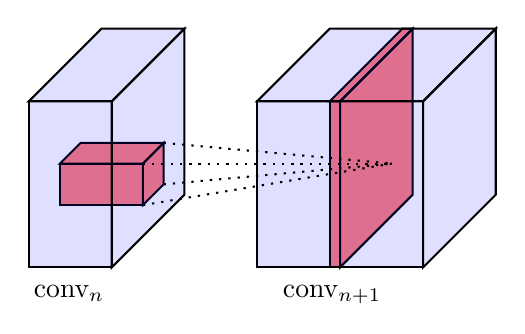
\begin{tikzpicture}[x=0.75pt,y=0.75pt,yscale=-1,xscale=1]
%uncomment if require: \path (0,300); %set diagram left start at 0, and has height of 300

%Shape: Rectangle [id:dp6024605162727454] 
\draw  [fill={rgb, 255:red, 255; green, 0; blue, 0 }  ,fill opacity=0.5 ] (65,55) -- (65,75) -- (55,85) -- (55,65) -- cycle ;
%Shape: Rectangle [id:dp3646079651688856] 
\draw  [fill={rgb, 255:red, 255; green, 0; blue, 0 }  ,fill opacity=0.5 ] (25,55) -- (65,55) -- (55,65) -- (15,65) -- cycle ;
%Shape: Rectangle [id:dp868859927177302] 
\draw  [fill={rgb, 255:red, 255; green, 0; blue, 0 }  ,fill opacity=0.5 ] (15,65) -- (55,65) -- (55,85) -- (15,85) -- cycle ;

%Shape: Rectangle [id:dp9640609623848294] 
\draw  [fill={rgb, 255:red, 255; green, 0; blue, 0 }  ,fill opacity=0.5 ] (150,115) -- (150,35) -- (185,0) -- (185,80) -- cycle ;
%Shape: Rectangle [id:dp7344880876209389] 
\draw  [fill={rgb, 255:red, 255; green, 0; blue, 0 }  ,fill opacity=0.5 ] (180,0) -- (185,0) -- (150,35) -- (145,35) -- cycle ;
%Shape: Rectangle [id:dp8025210042319197] 
\draw  [fill={rgb, 255:red, 255; green, 0; blue, 0 }  ,fill opacity=0.5 ] (150,35) -- (145,35) -- (145,115) -- (150,115) -- cycle ;
%Shape: Square [id:dp46929555136260237] 
\draw  [fill={rgb, 255:red, 0; green, 0; blue, 255 }  ,fill opacity=0.125 ] (110,35) -- (190,35) -- (190,115) -- (110,115) -- cycle ;
%Shape: Rectangle [id:dp925351136013279] 
\draw  [fill={rgb, 255:red, 0; green, 0; blue, 255 }  ,fill opacity=0.125 ] (225,0) -- (225,80) -- (190,115) -- (190,35) -- cycle ;
%Shape: Rectangle [id:dp2623353287641743] 
\draw  [fill={rgb, 255:red, 0; green, 0; blue, 255 }  ,fill opacity=0.125 ] (145,0) -- (225,0) -- (190,35) -- (110,35) -- cycle ;
%Shape: Rectangle [id:dp3905291664649332] 
\draw  [fill={rgb, 255:red, 0; green, 0; blue, 255 }  ,fill opacity=0.125 ] (35,0) -- (75,0) -- (40,35) -- (0,35) -- cycle ;
%Shape: Rectangle [id:dp6566535915239192] 
\draw  [fill={rgb, 255:red, 0; green, 0; blue, 255 }  ,fill opacity=0.125 ] (0,35) -- (40,35) -- (40,115) -- (0,115) -- cycle ;
%Straight Lines [id:da2237278586052034] 
\draw  [dash pattern={on 0.84pt off 2.51pt}]  (55,65) -- (175,65) ;
%Straight Lines [id:da7503402966926799] 
\draw  [dash pattern={on 0.84pt off 2.51pt}]  (65,55) -- (175,65) ;
%Straight Lines [id:da5706030328739486] 
\draw  [dash pattern={on 0.84pt off 2.51pt}]  (65,75) -- (175,65) ;
%Straight Lines [id:da5697803495881845] 
\draw  [dash pattern={on 0.84pt off 2.51pt}]  (55,85) -- (175,65) ;
%Shape: Rectangle [id:dp3678712110668708] 
\draw  [fill={rgb, 255:red, 0; green, 0; blue, 255 }  ,fill opacity=0.125 ] (75,0) -- (75,80) -- (40,115) -- (40,35) -- cycle ;

% Text Node
\draw (1,122.4) node [anchor=north west][inner sep=0.75pt]    {conv$_{n}$};
% Text Node
\draw (121,122.4) node [anchor=north west][inner sep=0.75pt]    {conv$_{n+1}$};
\end{tikzpicture}
\caption{Each kernel of a convolutional layer (in red) performs a convolution as a tensor-product at each spatial location of an incoming tensor, to produce a single channel of the output tensor.}
\label{fig:convolutional_layer}
\end{figure}

The first convolutional layers kernels were originally $6$ $5 \times 5$ kernels. The six convolutions are performed on the same input, producing six \emph{activation maps} that are concatenated across the channel dimension. As a result, the following convolutional layer originally had $16$ $5 \times 5 \times 6$ kernels. Notice the kernels are now tensors, so as to account for the multi-channel inputs. This represents a generalisation of Equation \ref{eq:convolution_operation} in which the each channel is convolved separately and the outputs are summed channel-wise. A depiction is given in Figure \ref{fig:convolutional_layer}.  

The maxpool are pooling layers (in effect max filter operations), replacing each $2\times2$ grid of pixels with their maxima. The maxpool operations are usually performed at a \emph{stride} of $2$, resulting in an output halved in each spatial dimension. This ensures the most salient features are routed to the proceeding layers.

After the final pooling operation, the input tensor is implicitly flattened and traverses a series of final, fully-connected layers. The fully-connected layers were originally of size $120$, $84$, and $10$ neurons, for the $10$-way classification of MNIST digits. Note the numbers are fairly arbitrary and partially reflect the computational budget of the day. The architecture can be understood as having a feature extraction component in the convolutional and pooling layers, and a classification component in the fully-connected layers, with all layers trained end-to-end in unison using backpropagation and gradient descent.

%$\mathbf{F}_1 \in \mathbb{R}^{120}$ concatenates the 16 activation maps of size $5\times5$ vector. The rest of the network is like a traditional fully-connected network with $\mathbf{F}_2 \in \mathbb{R}^{84}$ and a $10 \times 1$ output layer.

%* Note that the reduction in size after each convolution is due to convolutions not being performed at the borders (aka *valid* convolution). It is, however, more common to *pad* the input images with zeros to allow convolution on every pixel, thereby preserving the input size. In our model, we have $28 \times 28$ inputs that will be zero-padded.

% Datasets of similar resolution to MNIST, albeit in full RGB colour, are CIFAR10 (10 object classes) and CIFAR100 (100 object classes). These datasets tend to pose more of a challenge to object classifiers. For an example of training a deep network on these datasets, see \hyperref[https://github.com/jcboyd/vgg-fun]{https://github.com/jcboyd/vgg-fun}. Despite successes on isolated problems such as in \cite{matan1992reading}, the contemporary hardware was not powerful enough to drive neural networks to their full potential, and interest in them soon declined. Thus followed a second neural network winter\footnote{The first such winter occurred in the 1970s with the publication of ``Perceptrons'' by Minsky and Papert. This was a damning repudiation of the simple Perceptron networks designed by Frank Rosenblatt in 1957.} as researchers turned to models with more rigorous mathematical grounding, such as support vector machines. Nevertheless, the tenacity of deep learning to outperforms its competitors, particularly on image data, won it a minority of champions and defenders (see for example \cite{simard2003best}).

\subsection{AlexNet and the ConvNet revolution}

The emphatic victory of AlexNet (\cite{krizhevsky2012imagenet}) in the 2012 ImageNet Large Scale Visual Recognition Challenge (ILSVRC)\footnote{1000 classes, 1 million images} heralded the inexorable rise of CNNs. While emulating the same basic design as LeNet, the AlexNet architecture was deeper (more layers) and wider (more neurons/kernels), and processed larger images ($224\times224\times3$px), featuring in excess of $60$ million parameters over 8 learnable layers. The breakthrough of AlexNet is often attributed to the conjunction of three technological developments:

\begin{enumerate}
\item The rise of graphical processing units (GPUs)
\item The sourcing of large image datasets such as ImageNet
\item The streamlining of neural network training e.g. more stable activation functions (ReLU), adaptive optimisers, regularisers such as dropout, and better weight initialisation or pre-training strategies.
\end{enumerate}

With academic and industrial vision research in full swing, VGGNet\footnote{Visual Geometry Group at Oxford University.} and GoogLeNet were followed as ILSVRC 2014 frontrunners, pushing the state-of-the-art ever further, while achieving lasting fame. The competition winner, GoogLeNet, pioneered a more complex neural network design by engineering the \emph{inception module}, a concatenation of differently-sized convolutions. Laying several inception blocks end-to-end constitutes the 22-learnable-layer GoogLeNet. VGGNet likewise strived for unprecedented network depth (up to 19 learnable layers) while advocating some simple design principles. For example, (padded) $3\times 3$ convolutions are used everywhere, given that a stack of three $3 \times 3$ convolutions with $C$ channels has a receptive field of size $7 \times 7$ on its inputs, despite having $27C^2$ weights, fewer than a single $7 \times 7$ kernel at $49C^2$.

A multitude of network architectures have since been proposed. Among the most influential is ResNet, which introduced the residual block: a skip connection bypassing a stack convolutions. The motivation is to prevent the gradients of deeper layers from overwhelming all others early during training. The residual block thus facilitated the training of extremely deep networks of up to 1202 layers\footnote{However, the standard depths are 50, 101, and 152 layers.}. More recently, EfficientNet proposed a ``compound scaling'' design strategy to increase network depth, width, and resolution in unison to maximise the performance benefit. As of February 2020, the state-of-the-art in ImageNet is an EfficientNet variant. Table \ref{table:convnets} displays results from the history of the ILSVRC challenge illustrating the advancement of minimisation of test error over time. Note that AlexNet was evaluated on the ILSVRC 2012 dataset, whereas all others where evaluated on a similar dataset from the 2014 competition. Also, while GoogLeNet was the ILSVRC 2014 challenge winner, it prevailed only with a complex ensemble approach; we provide single-model results only. 

\begin{table}
\centering
\begin{tabular}{|c|c|c|c|c|} 
\hline
 Model & Year &  Top-1 & Top-5 & No. Parameters \\ 
 \hline
 AlexNet & $2012$ & $40.7\%$ & $18.2\%$ & $60$M \\
 GoogLeNet & $2014$ & - & $10.1\%$ & $6.8$M\\
 VGG-19 & $2014$ & $25.5\%$ & $8.0\%$ & $144$M \\
 ResNet-152 & $2015$ & $22.2\%$ & $6.2\%$ & $60$M \\
 EfficientNet & 2019 & $15.6\%$ & $2.9\%$ & $66$M \\
 \hline
\end{tabular}
\caption{Single-model test errors on ImageNet for five groundbreaking CNNs. Note AlexNet was evaluated on the ILSVRC 2012 dataset, the others on ILSVRC 2014. Human performance has been estimated to be $5\%$ Top-5 error (\cite{karpathy2014learned}).}
\label{table:convnets}
\end{table}

\section{Neural object detection}

% \tikzstyle{block} = [rectangle, draw, fill=blue!20, node distance=2.5cm,
%     text width=3.5em, text centered, rounded corners, minimum height=3em]
% \tikzstyle{line} = [draw, -latex']

An object detection system $f$ is a model or automated pipeline that both localises and classifies ontological objects in images. Localisation is usually expressed as a bounding box, which the detector emits along with the class prediction as the tuple,

\begin{equation}
f : \mathbf{x} \to \big\{(x, y, w, h, c)\big\},
\end{equation}

for image $\mathbf{x}$, where $x, y$ are the coordinates of the bounding box center, and $w, h$ are its width and height. The value $c$ denotes the class of the detected object. Figure \ref{fig:rcnn_ramen} illustrates a set of object detections made on a custom image by a state-of-the-art system.

\begin{figure}[h]
\centering
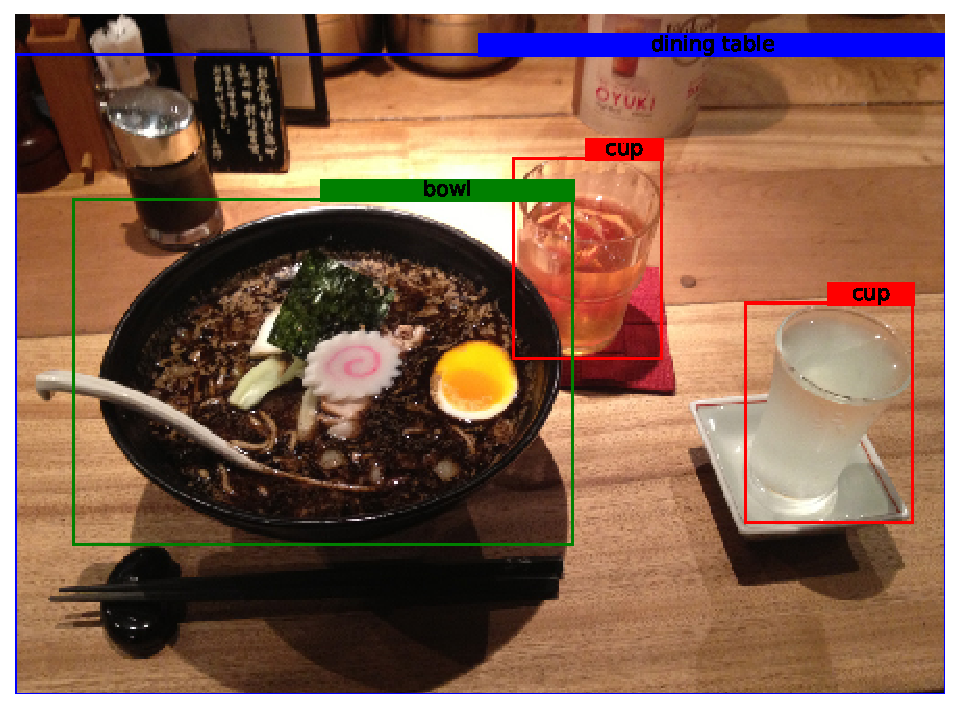
\includegraphics[width=\textwidth]{img/rcnn_ramen.pdf}
\caption{Object detections made by pre-trained R-CNN available in \texttt{PyTorch} (\cite{paszke2017automatic}). The image was taken in the Kyoto Gogyo ramen restaurant in Kyoto.}
\label{fig:rcnn_ramen}
\end{figure}

Whereas the ILSVRC datasets came to set the gold standard benchmarks in image classification, similarly rich datasets predominate for object detection. The Microsoft Common Objects in COntext (COCO) (\cite{lin2014microsoft}) (80 classes $+$ background) and the PASCAL\footnote{Pattern Analysis, Statistical Modelling and Computational Learning} Visual Object Classes (VOC) challenge (20 classes $+$ background) datasets (\cite{everingham2010pascal}) are the two leading datasets against which state-of-the-art object detection systems are tested.  Following the explosion of interest in CNNs as image classifiers in 2012, rapid progress was made virtually in parallel for neural object detectors. An early example is \emph{Overfeat} (\cite{sermanet2013overfeat})), appearing in 2013. The basic architecture of Overfeat was an AlexNet, refurbished as a fully-convolutional model\footnote{Replacing fully-connected with convolutional layers frees the network from the constraint of a fixed input size.}. 

No family of object detectors is more celebrated than the R-CNN series, however, the study of which is to be recommended to the pupil of deep learning.

\subsection{Regions with CNN features}

Regions with CNN features (R-CNN) (\cite{girshick2014rich}) began as a disjoint pipeline consisting of four ordered stages:

\begin{itemize}
\item[(1)] region proposal
\item[(2)] feature extraction,
\item[(3a)] object classification 
\item[(3b)] bounding box correction
\end{itemize}

In the earliest iterations of R-CNN, the ``selective search'' algorithm played the role of stage (1)\footnote{A greedy algorithm that progressively merges homogeneous regions of an input image, from which derive a large number of bounding box proposals.}. Feature extraction (2) was then performed by a pre-trained CNN, producing a ``CNN code'' feature vector for each region. Stage (3a) consisted of a set of linear models (typically SVMs) that perform one-vs-the-rest classification for each object class. These models were trained offline on the outputs of stage (2), ``warped'' to a standard size. Likewise, in stage (3b), a set of per-class (ridge) regression models are trained to correct the region proposal coordinates $(x, y, w, h)$.

In Fast R-CNN (\cite{girshick2015fast}) stages (3a) and (3b) were absorbed into the CNN ``backbone'' of stage (2) as appendages to the neural feature extractor trained end-to-end. Now, entire images were processed in a single forward pass, with the region proposals cropped from the activation maps. The encoded regions were quantised by a generalisation of the max pooling layer, RoIPool. Faster R-CNN \cite{ren2015faster} completed the work by integrating the region proposal algorithm (1) into the network. For this purpose, a separate region proposal network (RPN) was trained to predict both object presence and bounding box coordinates. A multi-stage training procedure was used to synchronise the weights between the two networks. Consequently, at prediction time, the feature extraction can be performed for both networks in a single forward pass. Then, the RPN heads produce the region proposals, which are passed to the heads of the R-CNN for detection. The overhead of region proposal is therefore negligible, and Faster R-CNN produces state-of-the-art object detection results more or less at real time.

% The synthesis of object detection and semantic segmentation is called \emph{instance segmentation}. Here, semantic objects are not only localised and classified, but also segmented as individual entities. This is the accomplishment of Mask R-CNN (\cite{he2017mask}), which extends Faster R-CNN by appending yet another branch for segmentation. In addition, the features are taken from different layers of the backbone and combined in a \emph{feature pyramid network} (\cite{lin2017feature}), as seen also in RetinaNet (\cite{lin2017focal}).

\section{Fighting overfitting in deep learning}

In machine learning, overfitting is the effect of \emph{fitting the noise instead of the signal}. In practice, all data contains noise obscuring the ground signal, and when a dataset is sufficiently small, a modestly powerful model may interpolate it perfectly, only to then be useless on test data. Much of machine learning is ultimately concerned with striking a balance between overfitting and underfitting. In supervised learning, this balance is evaluated with \emph{generalisation error}, the ability of the model to generalise the data, which is estimated by evaluating a trained model over a test set of independent, unseen data. The \emph{bias-variance decomposition} illustrates the tradeoff between over- and underfitting. Suppose we have $Y = f(x) + \epsilon$ generating training data with $f(x)$ the true signal for data point $x$, and noise, $\epsilon = \mathcal{N}(0, \sigma^2)$. Let our model estimate be denoted by $\hat{f}(x)$. Then, the MSE (here an arbitrary measure of goodness of fit) between an estimate and the true parameters, averaged over all possible data,

\begin{align}
\mathbb{E}[(Y - \hat{f}(x))^2] &= \mathbb{E}[((f(x) + \epsilon - \mathbb{E}[\hat{f}(x)]) + (\mathbb{E}[\hat{f}(x)] - \hat{f}(x)))^2] \\
&= \sigma^2 + \mathbb{E}[f(x) - \mathbb{E}[\hat{f}(x)]]^2 + \mathbb{E}[(\hat{f}(x) - \mathbb{E}[\hat{f}(x)])^2] \\
&= \text{noise} + \text{bias}^2 + \text{variance}
\end{align}

where in step (1.2) some terms are eliminated with zero mean. Note the positive terms means this represents a lower bound on error. The bias term represents underfitting as a simplified model fails to follow a more complex trend (for example a linear model undershooting a higher-order function). This bias will be observed in training error. The variance term represents overfitting as the model varies around its mean greatly to interpolate noisy data. This variance will be observed in test error.

Neural networks, being such powerful ``universal approximators'' (\cite{hornik1989multilayer}), are especially prone to overfitting. Many strategies to attenuate it have therefore been proposed. A common approach used elsewhere in machine learning is \emph{weight regularisation}, often called \emph{weight decay}. This usually takes the form of a square error penalty term in the loss function. Parametric models that overfit usually require large parameter values (in the extreme, a degree $n$ polynomial with up to $n-1$ turning points can interpolate $n+1$ data points), so regularisation curtails this tendency.

Deep learning succeeds because it embodies a different type of bias. Between layers of a vanilla fully-connected network, the number of weights is quadratic in the number of neurons per layer. Deep learning models reduce this dimensionality by spatial weight sharing, in the case of convolutional network, and weight sharing in time, in the case of recurrent neural networks. These may be referred to as \emph{structural biases}.

Other tricks to avoid overfitting include dropout (\cite{srivastava2014dropout}), whereby neurons are randomly zeroed-out during training so as to curtail complex co-dependencies; batch normalisation (\cite{ioffe2015batch}), where a normalisation operation is performed on the inputs of each layer so as to standardise their variance (and avoid ``internal covariate shift''); and data augmentation, which aims to increase the data supply. It is data augmentation that has particular relevance to this dissertation, and which we detail in the following.

%\begin{figure}
%\centering
%\begin{tabular}{cc}
%\subfloat[$k = 1$]{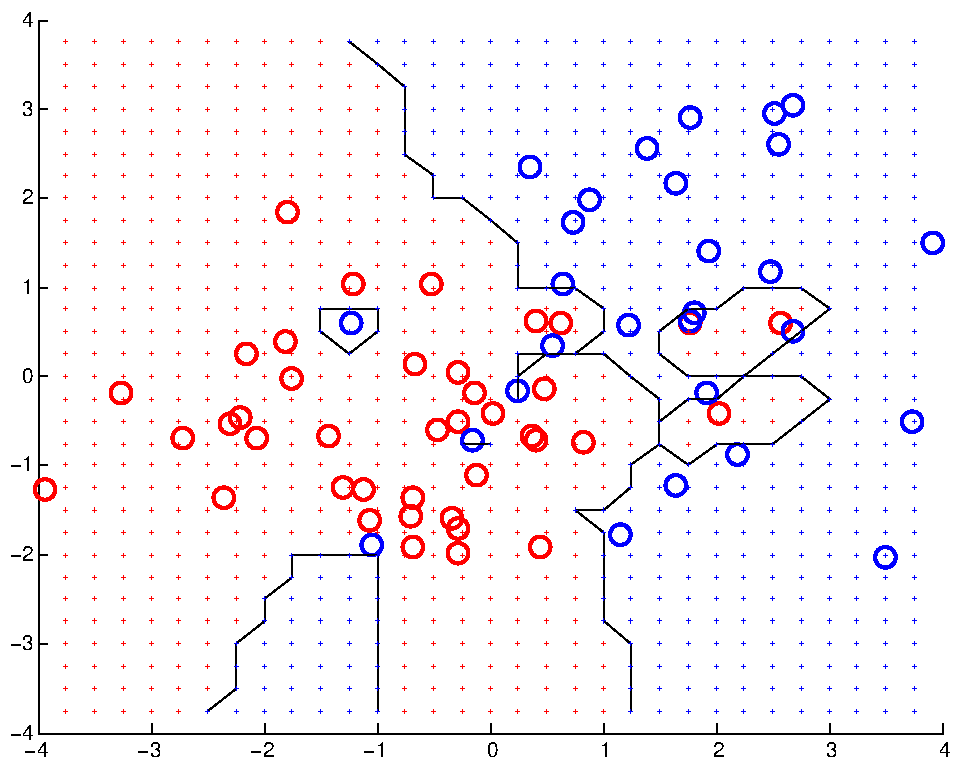
\includegraphics[width=0.5\textwidth]{Figures/knn1.pdf}} & 
%\subfloat[$k = 7$]{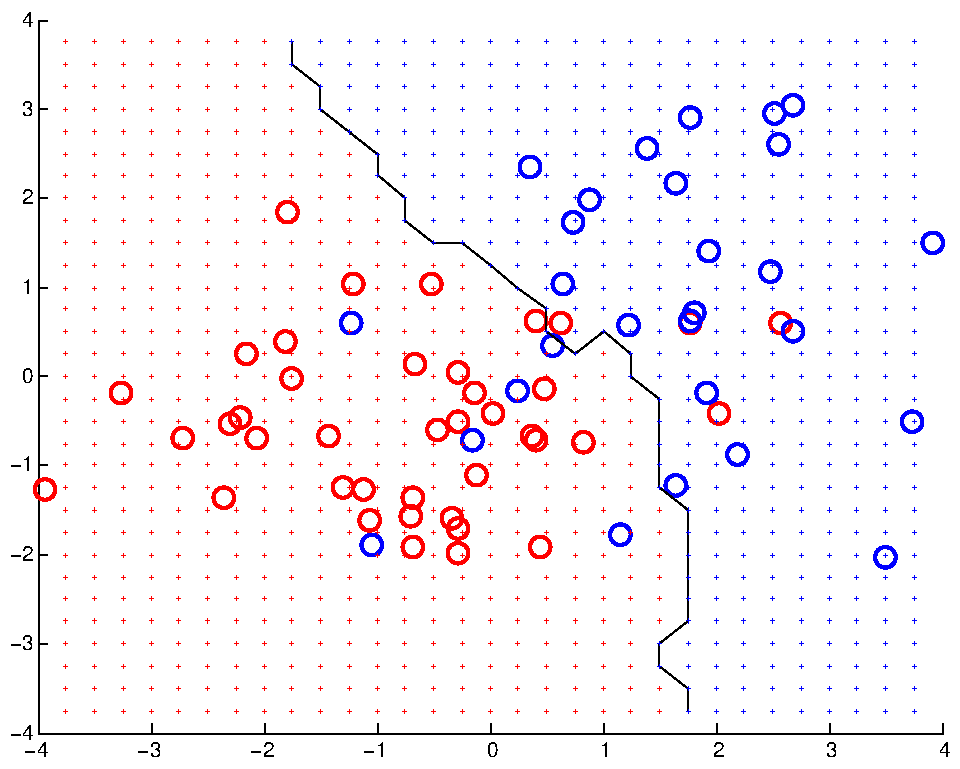
\includegraphics[width=0.5\textwidth]{Figures/knn7.pdf}}
%\end{tabular}
%\caption{Visualisation of overfitting with k-nearest neighbours (kNN) (non-parametric model). A data point is classified as the majority class of the $k$ geometrically closest data points. Note the steadier decision boundary formed for $k = 7$. This classifier can be very effective, but suffers from the curse of dimensionality. Data normalisation and dimensionality reduction usually help. However, in certain high-dimensional data sets where data is confined to a lower-dimensional manifold, for example in OCR data, kNN can be very effective. Unlike most classifiers, test time is much greater than training time. Approximations using memory tradeoffs mitigate this. Created with \texttt{knnDemo.m}.}
%\label{fig:knn}
%\end{figure}

\subsection{Data augmentation}

\begin{figure}[h]
\centering

\tikzset{every picture/.style={line width=0.75pt}} %set default line width to 0.75pt        

\begin{tikzpicture}[x=0.75pt,y=0.75pt,yscale=-1,xscale=1]
%uncomment if require: \path (0,267); %set diagram left start at 0, and has height of 267

%Image [id:dp4690746643617628] 
\draw (305,135) node  {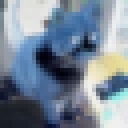
\includegraphics[width=37.5pt,height=37.5pt]{img/augmentation_cat_aug2.png}};
%Shape: Rectangle [id:dp5844515089762182] 
\draw   (280,110) -- (330,110) -- (330,160) -- (280,160) -- cycle ;

%Image [id:dp8031263564437391] 
\draw (215,175) node  {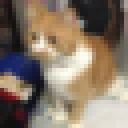
\includegraphics[width=37.5pt,height=37.5pt]{img/augmentation_cat.png}};
%Shape: Rectangle [id:dp007056558703781413] 
\draw   (190,150) -- (240,150) -- (240,200) -- (190,200) -- cycle ;

%Image [id:dp08461336687255161] 
\draw (115,95) node  {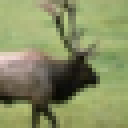
\includegraphics[width=37.5pt,height=37.5pt]{img/augmentation_deer.png}};
%Shape: Rectangle [id:dp6749055875742906] 
\draw   (90,70) -- (140,70) -- (140,120) -- (90,120) -- cycle ;

%Image [id:dp464239246082056] 
\draw (435,115) node  {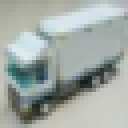
\includegraphics[width=37.5pt,height=37.5pt]{img/augmentation_truck.png}};
%Shape: Rectangle [id:dp39795630279129157] 
\draw   (410,90) -- (460,90) -- (460,140) -- (410,140) -- cycle ;

%Image [id:dp24631782250209233] 
\draw (395,175) node  {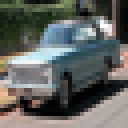
\includegraphics[width=37.5pt,height=37.5pt]{img/augmentation_car.png}};
%Shape: Rectangle [id:dp6628152059484871] 
\draw   (370,150) -- (420,150) -- (420,200) -- (370,200) -- cycle ;

%Image [id:dp8576511044757406] 
\draw (65,155) node  {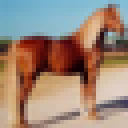
\includegraphics[width=37.5pt,height=37.5pt]{img/augmentation_horse.png}};
%Shape: Rectangle [id:dp827131947184459] 
\draw   (40,130) -- (90,130) -- (90,180) -- (40,180) -- cycle ;

%Image [id:dp9366678348308388] 
\draw (265,75) node  {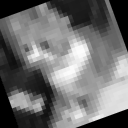
\includegraphics[width=37.5pt,height=37.5pt]{img/augmentation_cat_aug1.png}};
%Shape: Rectangle [id:dp2003057013901418] 
\draw   (240,50) -- (290,50) -- (290,100) -- (240,100) -- cycle ;

%Shape: Sine Wave Form [id:dp44457004411395107] 
\draw   (20,139.57) .. controls (113.59,0.73) and (157.72,0) .. (249.97,139.57) .. controls (342.28,279.14) and (385.54,280) .. (480,139.57) ;
%Shape: Circle [id:dp6762877746787627] 
\draw  [fill={rgb, 255:red, 208; green, 2; blue, 27 }  ,fill opacity=1 ] (34,112) .. controls (34,108.69) and (36.69,106) .. (40,106) .. controls (43.31,106) and (46,108.69) .. (46,112) .. controls (46,115.31) and (43.31,118) .. (40,118) .. controls (36.69,118) and (34,115.31) .. (34,112) -- cycle ;
%Shape: Circle [id:dp8216805850204476] 
\draw  [fill={rgb, 255:red, 208; green, 2; blue, 27 }  ,fill opacity=1 ] (68,70) .. controls (68,66.69) and (70.69,64) .. (74,64) .. controls (77.31,64) and (80,66.69) .. (80,70) .. controls (80,73.31) and (77.31,76) .. (74,76) .. controls (70.69,76) and (68,73.31) .. (68,70) -- cycle ;
%Shape: Circle [id:dp5289135761245862] 
\draw  [fill={rgb, 255:red, 208; green, 2; blue, 27 }  ,fill opacity=1 ] (244.97,140.57) .. controls (244.97,137.26) and (247.66,134.57) .. (250.97,134.57) .. controls (254.28,134.57) and (256.97,137.26) .. (256.97,140.57) .. controls (256.97,143.88) and (254.28,146.57) .. (250.97,146.57) .. controls (247.66,146.57) and (244.97,143.88) .. (244.97,140.57) -- cycle ;
%Shape: Circle [id:dp5124108509736214] 
\draw  [fill={rgb, 255:red, 74; green, 144; blue, 226 }  ,fill opacity=1 ] (233,122) .. controls (233,118.69) and (235.69,116) .. (239,116) .. controls (242.31,116) and (245,118.69) .. (245,122) .. controls (245,125.31) and (242.31,128) .. (239,128) .. controls (235.69,128) and (233,125.31) .. (233,122) -- cycle ;
%Shape: Circle [id:dp3304180493841744] 
\draw  [fill={rgb, 255:red, 74; green, 144; blue, 226 }  ,fill opacity=1 ] (257,159) .. controls (257,155.69) and (259.69,153) .. (263,153) .. controls (266.31,153) and (269,155.69) .. (269,159) .. controls (269,162.31) and (266.31,165) .. (263,165) .. controls (259.69,165) and (257,162.31) .. (257,159) -- cycle ;
%Shape: Circle [id:dp5055457984695153] 
\draw  [fill={rgb, 255:red, 208; green, 2; blue, 27 }  ,fill opacity=1 ] (426,204) .. controls (426,200.69) and (428.69,198) .. (432,198) .. controls (435.31,198) and (438,200.69) .. (438,204) .. controls (438,207.31) and (435.31,210) .. (432,210) .. controls (428.69,210) and (426,207.31) .. (426,204) -- cycle ;
%Shape: Circle [id:dp11055235341340652] 
\draw  [fill={rgb, 255:red, 208; green, 2; blue, 27 }  ,fill opacity=1 ] (455,167) .. controls (455,163.69) and (457.69,161) .. (461,161) .. controls (464.31,161) and (467,163.69) .. (467,167) .. controls (467,170.31) and (464.31,173) .. (461,173) .. controls (457.69,173) and (455,170.31) .. (455,167) -- cycle ;
\end{tikzpicture}
\caption{Data augmentation can make modest but useful interpolations of the space surrounding real images. CIFAR-10 images marked by red circle; augmented images marked by blue circle; black line represents natural image manifold. Upper augmentation based on conversion to grayscale (an element-wise weighted average of the RGB pixels) and rotation; the lower on colour inversion and horizontal flipping.}
\label{fig:augmentation}
\end{figure}

In the long run, as more data is added, a model with sufficient capacity improves its predictive power (generalisation error). In an ideal world, our data is unlimited. However, annotated data for supervised training is expensive, requiring manual effort, often by domain experts. Data augmentation is a technique for obtaining new data fighting overfitting in machine learning models thereby improving generalisation (test time) error (\cite{shorten2019survey}). The idea is to extract additional data \emph{gratis} from the available dataset, by means of bootstrapping or interpolation. A classic algorithm is SMOTE (Synthetic Minority Over-sampling TechniquE) (\cite{chawla2002smote}), which interpolates lines between training samples and their nearest neighbours in feature space, to create synthetic points, and as an alternative to over-sampling by replacement.

Data augmentation is especially vital in deep learning, where powerful neural networks require large datasets to train. Due to the geometry of natural images (pixels are ordered and neighbouring pixels are highly correlated), image data is uniquely receptive to data augmentation, and humans are well-equipped for the engineering of it. Images support a multitude of \emph{label-preserving transformations}, that is, transformations of lower-level image properties that nevertheless maintain the high-level semantic content. Examples are cropping, flipping, rotating, noise injection, convolution, and colour space transformations (if colour is available). These may be referred to as basic image manipulations (\cite{shorten2019survey}) and can be ``stacked'' (combined) endlessly, especially on the fly during training. Classic examples include image warping \cite{lecun1998gradient}, elastic deformations \cite{simard2003best}, and PCA-based colour space transformation \cite{krizhevsky2012imagenet}. However, data augmentation must not be mistaken as equivalent to adding authentic and may reinforce existing biases in a dataset (\cite{shorten2019survey}). The augmented images are highly interdependent and will not in general amount to substantially increasing the coverage of space of all images (see Figure \ref{fig:augmentation}). Additionally, certain transformations will be domain-specific. For example, biomedical imagery can usually be rotated arbitrarily without losing meaning, unlike images of everyday objects or handwritten digits.

Deep learning itself can be used as a powerful, albeit expensive, mode of data augmentation. One good example is \emph{adversarial training}. \cite{goodfellow2014explaining} show how with a precise perturbation to a model input, one may ``fool'' a linear model or neural network alike. Consider perturbing model input $\mathbf{x}$,

\begin{equation}
\hat{\mathbf{x}} = \mathbf{x} + \alpha\cdot\eta,
\end{equation}

where $\eta = \text{sign}(\mathbf{w})$ for $\mathbf{w}$ are the model weights of a softmax regression model and $\alpha$ a tuning parameter. Now, the model will predict $\sigma(\mathbf{w}^T\hat{\mathbf{x}}) = \sigma(\mathbf{w}^T\mathbf{x} + \alpha\cdot||\mathbf{w}||_1)$. If $\mathbf{x}$ is sufficiently high-dimensional (as image data often is) the perturbations will accumulate even for $\alpha << 1$ and can change the decision of the model. This produces a paradox especially apparent for image data: one may, for example, add a small, carefully chosen value to each pixel of an image, and the model may suddenly predict the wrong object class with high confidence, even though the perturbation is imperceptible to the human eye. This paradox defies intuitions about how neural networks represent images and ``adversarial attacks'' remain problematic for deep learning. \cite{goodfellow2014explaining} nevertheless showed how adversarial attacks could be harnessed during training to strengthen neural networks against such attacks, in effect a sort of data augmentation.

Generative models, in particular generative adversarial models (GANs) (\cite{goodfellow2014generative}) (loosely related to the above) are a more recent and exciting prospect for data augmentation. Generative models are trained to learn (perhaps implicitly) the data-generating distribution, and thereupon may be used as a sampling system for synthetic data. Ideally, a generative model based on deep neural networks will make for a more powerful interpolation system than any of the above.

One may also consider transfer learning as a form of data augmentation commuted via pretrained model. The information content of a rich source dataset $\mathcal{D}_S$ may be distilled by a powerful neural network, and transferred to augment the available data for learning some task on a target dataset $\mathcal{D}_T$. Indeed, style transfer involving deep, pretrained networks \cite{gatys2016image} is a powerful mode of data augmentation, as we discover in Chapter \ref{Chapter6}.

\section{Transfer learning}

Transfer learning is a set of solutions for learning problems in which training and test data differ in their marginal distribution, or else that the learning tasks differ between model training and testing (\cite{pan2009survey}). As such, these problems violate the basic assumption for training supervised models. Transfer learning bridges \emph{domains} of learning. A domain $\mathcal{D}$ consists of a feature space $\mathcal{X}$ and marginal probability distribution on that domain $P(X)$. A learning \emph{task} $\mathcal{T}$ is performed on a domain, itself consisting of a label space $\mathcal{Y}$ and some (usually unobserved) objective function $f(\cdot)$. In transfer learning problems we denote source domain and tasks $\mathcal{D}_S$ and $\mathcal{T}_S$ and likewise for target domain $\mathcal{D}_T$ and $\mathcal{T}_T$. The source is the data on which the model is initially trained, and the target is that for which it must be adapted.

\begin{figure}
\tikzset{every picture/.style={line width=0.75pt}} %set default line width to 0.75pt        

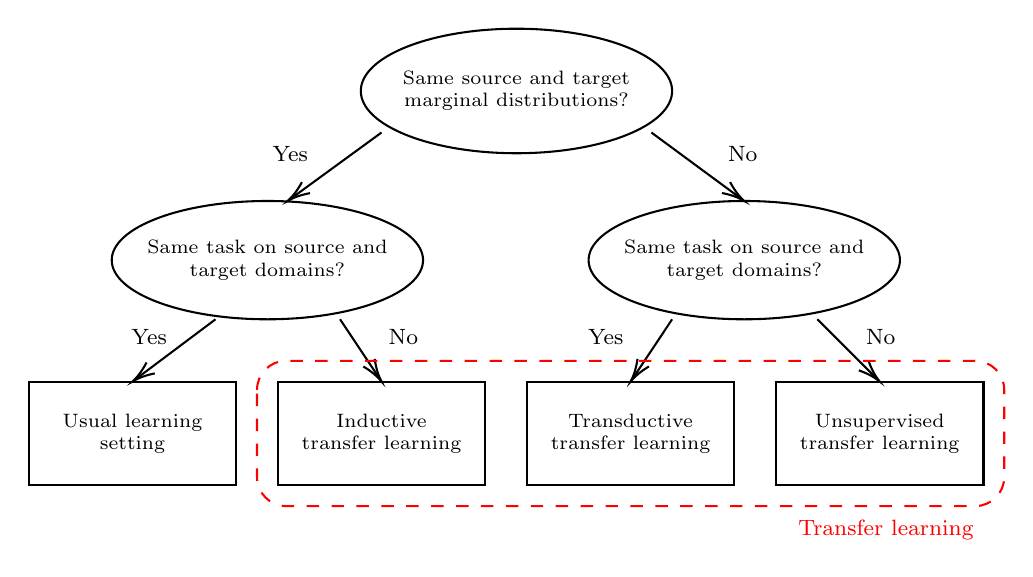
\begin{tikzpicture}[x=0.75pt,y=0.75pt,yscale=-1,xscale=1]
%uncomment if require: \path (0,269); %set diagram left start at 0, and has height of 269

%Shape: Ellipse [id:dp0974795717337551] 
\draw   (160,40) .. controls (160,23.43) and (193.58,10) .. (235,10) .. controls (276.42,10) and (310,23.43) .. (310,40) .. controls (310,56.57) and (276.42,70) .. (235,70) .. controls (193.58,70) and (160,56.57) .. (160,40) -- cycle ;
%Shape: Ellipse [id:dp9862877791048306] 
\draw   (40,121.5) .. controls (40,105.76) and (73.58,93) .. (115,93) .. controls (156.42,93) and (190,105.76) .. (190,121.5) .. controls (190,137.24) and (156.42,150) .. (115,150) .. controls (73.58,150) and (40,137.24) .. (40,121.5) -- cycle ;
%Shape: Ellipse [id:dp314231133167162] 
\draw   (269.75,121.5) .. controls (269.75,105.76) and (303.33,93) .. (344.75,93) .. controls (386.17,93) and (419.75,105.76) .. (419.75,121.5) .. controls (419.75,137.24) and (386.17,150) .. (344.75,150) .. controls (303.33,150) and (269.75,137.24) .. (269.75,121.5) -- cycle ;
%Shape: Rectangle [id:dp9001687557476825] 
\draw   (0,180) -- (100,180) -- (100,230) -- (0,230) -- cycle ;
%Shape: Rectangle [id:dp37462803697884417] 
\draw   (120,180) -- (220,180) -- (220,230) -- (120,230) -- cycle ;
%Shape: Rectangle [id:dp41799431397747233] 
\draw   (240,180) -- (340,180) -- (340,230) -- (240,230) -- cycle ;
%Shape: Rectangle [id:dp7754162600589308] 
\draw   (360,180) -- (460,180) -- (460,230) -- (360,230) -- cycle ;
%Straight Lines [id:da9176701651556409] 
\draw    (170,60) -- (126.37,91.82) ;
\draw [shift={(124.75,93)}, rotate = 323.9] [color={rgb, 255:red, 0; green, 0; blue, 0 }  ][line width=0.75]    (10.93,-3.29) .. controls (6.95,-1.4) and (3.31,-0.3) .. (0,0) .. controls (3.31,0.3) and (6.95,1.4) .. (10.93,3.29)   ;
%Straight Lines [id:da25605932186071767] 
\draw    (300,60) -- (343.14,91.81) ;
\draw [shift={(344.75,93)}, rotate = 216.41] [color={rgb, 255:red, 0; green, 0; blue, 0 }  ][line width=0.75]    (10.93,-3.29) .. controls (6.95,-1.4) and (3.31,-0.3) .. (0,0) .. controls (3.31,0.3) and (6.95,1.4) .. (10.93,3.29)   ;
%Straight Lines [id:da5288229165358177] 
\draw    (90,150) -- (51.6,178.8) ;
\draw [shift={(50,180)}, rotate = 323.13] [color={rgb, 255:red, 0; green, 0; blue, 0 }  ][line width=0.75]    (10.93,-3.29) .. controls (6.95,-1.4) and (3.31,-0.3) .. (0,0) .. controls (3.31,0.3) and (6.95,1.4) .. (10.93,3.29)   ;
%Straight Lines [id:da9359408976926888] 
\draw    (150,150) -- (168.89,178.34) ;
\draw [shift={(170,180)}, rotate = 236.31] [color={rgb, 255:red, 0; green, 0; blue, 0 }  ][line width=0.75]    (10.93,-3.29) .. controls (6.95,-1.4) and (3.31,-0.3) .. (0,0) .. controls (3.31,0.3) and (6.95,1.4) .. (10.93,3.29)   ;
%Straight Lines [id:da3772543817005427] 
\draw    (310,150) -- (291.11,178.34) ;
\draw [shift={(290,180)}, rotate = 303.69] [color={rgb, 255:red, 0; green, 0; blue, 0 }  ][line width=0.75]    (10.93,-3.29) .. controls (6.95,-1.4) and (3.31,-0.3) .. (0,0) .. controls (3.31,0.3) and (6.95,1.4) .. (10.93,3.29)   ;
%Straight Lines [id:da11594261351341528] 
\draw    (380,150) -- (408.59,178.59) ;
\draw [shift={(410,180)}, rotate = 225] [color={rgb, 255:red, 0; green, 0; blue, 0 }  ][line width=0.75]    (10.93,-3.29) .. controls (6.95,-1.4) and (3.31,-0.3) .. (0,0) .. controls (3.31,0.3) and (6.95,1.4) .. (10.93,3.29)   ;
%Rounded Rect [id:dp8619685472332226] 
\draw  [color={rgb, 255:red, 255; green, 0; blue, 0}  ,draw opacity=1 ][dash pattern={on 4.5pt off 4.5pt}] (110,184) .. controls (110,176.27) and (116.27,170) .. (124,170) -- (456,170) .. controls (463.73,170) and (470,176.27) .. (470,184) -- (470,226) .. controls (470,233.73) and (463.73,240) .. (456,240) -- (124,240) .. controls (116.27,240) and (110,233.73) .. (110,226) -- cycle ;
% Text Node
\draw (235,40) node  [font=\scriptsize] [align=center] {
Same source and target\\marginal distributions?
};
% Text Node
\draw (344.75,121.5) node  [font=\scriptsize] [align=center] {
Same task on source and\\target domains?
};
% Text Node
\draw (115,121.5) node  [font=\scriptsize] [align=center] {
Same task on source and\\target domains?
};
% Text Node
\draw (50,205) node  [font=\scriptsize] [align=center] {
Usual learning\\setting
};
% Text Node
\draw (170,205) node  [font=\scriptsize] [align=center] {
Inductive\\transfer learning
};
% Text Node
\draw (290,205) node  [font=\scriptsize] [align=center] {
Transductive\\transfer learning
};
% Text Node
\draw (410,205) node  [font=\scriptsize] [align=center] {
Unsupervised\\transfer learning
};
% Text Node
\draw (126,70.5) node  [font=\footnotesize] [align=left] {Yes};
% Text Node
\draw (344,70.5) node  [font=\footnotesize] [align=left] {No};
% Text Node
\draw (58,158.5) node  [font=\footnotesize] [align=left] {Yes};
% Text Node
\draw (410.5,158.5) node  [font=\footnotesize] [align=left] {No};
% Text Node
\draw (180.5,158.5) node  [font=\footnotesize] [align=left] {No};
% Text Node
\draw (278,158.5) node  [font=\footnotesize] [align=left] {Yes};
% Text Node
\draw (413,251.5) node  [font=\footnotesize,color={rgb, 255:red, 255; green, 0; blue, 0 }  ,opacity=1 ] [align=left] {Transfer learning};
\end{tikzpicture}
\caption{Positioning transfer learning with respect to the typical learning setting. Categories of transfer learning differ either with respect to the marginal distribution. Reproduced from https://en.wikipedia.org/wiki/Domain\_adaptation}
\label{fig:transfer_modes}
\end{figure}

Neural networks, with their endless flexibility, are well-equipped for transfer learning. Shortly after the deep learning revolution in 2012, the potential for the learning transfer of powerful pretrained neural networks was discovered (see \cite{zeiler2014visualizing} and \cite{sharif2014cnn}). Pretrained networks are often used in one of two ways:

\begin{enumerate}
\item feature extraction: a pretrained network is used to extract features for a new problem by passing images forward through its hidden layers and recording a given layer (``CNN code'') as a vector of (obscure) image features.
\item fine-tuning: a pretrained network recommences training on a new problem from the previous point of convergence, usually at a significantly lower learning rate, and often only on the deepest layers.
\end{enumerate}

The pretraining itself is usually done on a large standard image corpus like ImageNet. The success of these approaches illustrates the universality of the filters learned by deep networks, as general feature extractors for images. Neither approach fits easily into the schema of Figure \ref{fig:transfer_modes}. However, if the target images are similar in resolution and content, for example, the low-level neural activity of earlier layers may be identical to the source dataset, placing it near inductive transfer learning.

An interesting way to perform transductive transfer with deep learning is with \emph{domain-adversarial neural networks}, which we describe presently.

\subsection{Domain-adversarial neural networks}
\label{subsubsec:adversarial_notes}

% We are here concerned with unsupervised domain adaptation. That is, domain adaptation between source $S = \{(\mathbf{x}_i, y_i)\} \sim \mathcal{D}_S$ and target $T = \{\mathbf{x}_i\} \sim \mathcal{D}_T$ datasets, noting the target is \emph{unlabelled} (unsupervised), or partially labelled (semi-supervised). 

The inspiration for domain-adversarial neural networks (DANNs) lies in work published in \cite{ben2010theory}, which defines the $\mathcal{H}$-divergence,

\begin{equation}
d_\mathcal{H}(D_S^X, D_T^X) = 2\sup_{h \in \mathcal{H}}\Big|P_{\mathbf{x} \sim D_S^X}\big(h(\mathbf{x})= 1\big) - P_{\mathbf{x} \sim D_T^X}\big(h(\mathbf{x}) = 1\big)\Big|,
\end{equation}

that is, given a source domain (distribution), $D_S^X$ (marginalised by the input variable), and a target domain $D_T^X$, and given a hypothesis class\footnote{Category of classifiers, e.g. linear SVMs.} $\mathcal{H}$, the divergence between the source and target domains with respect to $\mathcal{H}$ is the classifier (here binary--for simplicity) that, proportionally, most classifies the domains into separate classes.

To illustrate, suppose we choose our hypothesis class to be a linear SVM. This class is capable (through choice of the SVM weights) of creating any possible linear hyperplane. Suppose the two domains were linearly separate in the feature space (see Figure \ref{fig:divergence}). It would then be possible to train an SVM to perfectly separate the two, putting one domain fully into the positive class, and the other into the negative class. This would maximise the inner expression of the divergence formula, thus describing a high divergence. Should we have, on the other hand, two highly overlapping domains, any hyperplane cut through the middle of the point cloud would give us a divergence close to 0. Should we cut so as to isolate a few outlier points of a particular class, these would represent only a small proportion of the data, and the probability would also be close to 0. Intuitively, the $\mathcal{H}$-divergence captures the effect nicely.

\begin{figure}[!ht]
\centering
    \subfloat[Low divergence\label{fig:divergence_a}]{
        \begin{tikzpicture}[>=stealth',x=0.9cm,y=0.9cm]
            \draw (0,0) rectangle (6,6);
            % \draw dashed line
            \draw[dashed]  (1,5.9) -- (4.5,0.1);
            \draw[dashed]  (0.1,3) -- (5.9, 3);
            \draw[dashed]  (0.1,0.1) -- (5.9, 5);

            \def\positive{{
            {4.3,3.3},{4,.8},{3.5,2},{2.2,4.1},{2.8,.8},{3,5.5},{3.2,5},
            {3.75,2.2},{3,4.2},{5, 0.5},{2.5,3},{4.3,.5}}}
            % \draw positive dots
            \foreach \i in {0,...,10} {
              \pgfmathparse{\positive[\i][0]}\let \x \pgfmathresult;
              \pgfmathparse{\positive[\i][1]}\let \y \pgfmathresult;
              \fill[black] (\x,\y) circle (2pt);
            }
            \def\negative{{
            {3.75,3},{2.5,5},{1.6,1.6},{4.5,5.2},{2.5,3.7},{3.9,4.7},{3,2.7},
            {3.5,1.2},{4.8,.9}}}
            % \draw negative dots
            \foreach \i in {0,...,8} {
              \pgfmathparse{\negative[\i][0]}\let \x \pgfmathresult;
              \pgfmathparse{\negative[\i][1]}\let \y \pgfmathresult;
              \draw[black] (\x,\y) circle (3pt);
            }
            \end{tikzpicture}
    }
    \qquad
    \subfloat[High divergence\label{fig:divergence_b}]{
        \begin{tikzpicture}[>=stealth',x=0.9cm,y=0.9cm]
            \draw (0,0) rectangle (6,6);
            % \draw line
%            \draw[color=red,line width=2pt] (1.5,5.9) -- (5,0.1);
%            % \draw dashed line
%            \draw[dashed]  (1,5.9) -- (4.5,0.1);
%            \draw[dashed]  (2,5.9) -- (5.5,0.1);
			\draw[dashed]  (1.5,5.9) -- (5,0.1);
%
            \def\positive{{
            {2.3,3.3},{4,.8},{1.5,2},{0.2,4.1},{1.8,.8},{1,5.5},{1.2,5},
            {0.75,.2},{2,4.2},{5, 0.5},{1.5,3},{2.3,.5}}}
            % \draw positive dots
            \foreach \i in {0,...,10} {
              \pgfmathparse{\positive[\i][0]}\let \x \pgfmathresult;
              \pgfmathparse{\positive[\i][1]}\let \y \pgfmathresult;
              \fill[black] (\x,\y) circle (2pt);
            }
            \def\negative{{
            {3.75,3},{3.5,5},{4.6,1.6},{4.5,5.2},{5.5,3.7},{3.9,4.7},{5,2.7},
            {3.5,4.2},{5.8,.9}}}
            % \draw negative dots
            \foreach \i in {0,...,8} {
              \pgfmathparse{\negative[\i][0]}\let \x \pgfmathresult;
              \pgfmathparse{\negative[\i][1]}\let \y \pgfmathresult;
              \draw[black] (\x,\y) circle (3pt);
            }
        \end{tikzpicture}
    }
    \caption{Overlapping domains (a) and divergent domains separated by a linear decision boundary (b). Modified from http://blog.pengyifan.com/tikz-example-kernel-trick/.}
    \label{fig:divergence}
\end{figure}


Conveniently, it is possible to compute a consistent estimate of the $\mathcal{H}$-divergence using finite data with the \emph{empirical} $\mathcal{H}$-divergence,

\begin{equation}
\hat{d}_\mathcal{H}(S, T) = 2\Bigg(1 - \min_{h \in \mathcal{H}}\bigg[\frac{1}{n}\sum_{i=1}^n\mathbf{1}[h(\mathbf{x}_i) = 0] + \frac{1}{n'}\sum_{i=n+1}^N\mathbf{1}[h(\mathbf{x}_i) = 1]\bigg]\Bigg)
\end{equation}

for samples, $S \sim D_S^X$ of size $n$ and $T \sim D_T^X$ of size $n'$. For convenience, these are indexed from $1\to n$ and $(n + 1) \to N$, where $N = n + n'$. Though this may be hard to compute precisely in general, we can approximate this simply by training a classifier of the class $\mathcal{H}$ on the constructed dataset, $U = \{(\mathbf{x}, 0) : \mathbf{x} \in S\} \cup \{(\mathbf{x}, 1) : \mathbf{x} \in T\}$, that is, a classifier to differentiate between the domains. The estimated generalisation error, $\epsilon$ of this classifier could then be used to approximate the empirical domain divergence as $2(1 - 2\epsilon)$.

\cite{ajakan2014domain} first formulate a DANN as a learning model of the form,

\begin{equation}
E(\theta_f, \theta_d, \theta_y) = \frac{1}{n}\sum_{i=1}^n\mathcal{L}_y^i(G_y(G_f(\mathbf{x} ; \theta_f) ; \theta_y), y_i) + \lambda R(\theta_f, \theta_d)
\end{equation}

where the $G_f$ component acts as a feature extractor, and $G_y$ is a classifier. These may have any neural architecture, shallow, deep, convolutional, etc. Recalling that the target data is unlabelled, they propose to define the regulariser of this model as,


\begin{equation}
R(\theta_f, \theta_d) = -\frac{1}{n}\sum_{i=1}^n\mathcal{L}_d^i(\theta_d, d_i) -\frac{1}{n'}\sum_{i=n+1}^N\mathcal{L}_d^i(\theta_d, d_i)
\end{equation}

where $\mathcal{L}_d^i(\theta_d, d^i) = \mathcal{L}(G_d(G_f(\theta_f) ; \theta_d), d_i), d_i \in \{0, 1\}$. Thus formulated, we have a loss maximising the negative of the minimisation term in the divergence formula. Therefore, adding this regulariser to the objective function, and maximising the objective with respect to its parameters, $\theta_d$, give a worse overall loss. At the same time, however, the feature parameters, $\theta_f$, which are trained to minimise the objective, are chosen to minimise this maximisation of the regulariser by the divergence parameters, $\theta_d$, thus maximising the minimising component of the divergence, thereby minimising the divergence. The feature parameters therefore play a dual role in both minimising classification loss, and minimising divergence (equivalently, maximising discrimination error), \emph{adversarially} to the domain classifier. This promotes domain invariant features. Formally, we have,

\begin{align}
(\theta_f, \theta_y) &= \arg\min_{\theta_f, \theta_y} E(\theta_f, \theta_y, \hat{\theta}_d) \notag \\
\theta_d &= \arg\max_{\theta_d} E(\hat{\theta}_f, \hat{\theta}_y, \theta_d)
\end{align}

which can be found as a saddle point of the update steps,

\begin{align}
\theta_f &\leftarrow \theta_f - \mu\Bigg(\frac{\partial \mathcal{L}_y^i}{\partial\theta_f} - \lambda\frac{\partial \mathcal{L}_d^i}{\partial\theta_f}\Bigg) \notag \\
\theta_y &\leftarrow \theta_f - \mu\frac{\partial \mathcal{L}_y^i}{\partial\theta_y} \notag \\
\theta_d &\leftarrow \theta_f - \mu\frac{\partial \mathcal{L}_d^i}{\partial\theta_d}
\end{align}

Note that $\theta_f$ is updated to minimise the classification loss, but maximise the domain classification loss. This is called the adversarial step. The main contribution of \cite{ganin2014unsupervised} is to apply this to deeper architectures (in particular, convolutional), and to introduce a ``gradient reversal layer'' to enable a smooth implementation without altering the internal implementations of gradient descent (this still assumes that the local gradients can be specified arbitrarily). This is achieved with the pseudo-function,

\begin{equation}
R_\lambda(\mathbf{x}) = \mathbf{x}
\end{equation}

whose gradient is hard-coded as,

\begin{equation}
\frac{\partial R_\lambda}{\partial\mathbf{x}} = -\lambda\mathbf{I}
\end{equation}

This pseudo-layer is inserted between the feature extractor and the domain classifier in the model formulation. It should be emphasised that this is not a mathematical trick, but rather an implementation hack. The gradient reversal layer is easy to implement in all the major deep learning frameworks.

\section{Generative adversarial networks}

Generative adversarial networks (GANs) (\cite{goodfellow2014generative}) is a learning framework that trains a generator model to be capable of sampling new data from a data distribution (in particular, images), learnt (implicitly) from a training set. GANs compete with variational autoencoders (\cite{kingma2013auto}) and, more recently, autoregressive models (\cite{oord2016pixel}) for image generation. We select GANs as the primary tool for our work in image synthesis in this dissertation, given their rich literature and versatility (as we shall soon see).

\begin{figure}
\centering
\tikzset{every picture/.style={line width=0.75pt}} %set default line width to 0.75pt        

\begin{tikzpicture}[x=0.75pt,y=0.75pt,yscale=-1,xscale=1]
%uncomment if require: \path (0,300); %set diagram left start at 0, and has height of 300

%Image [id:dp4196394413247667] 
\draw (280,180) node  {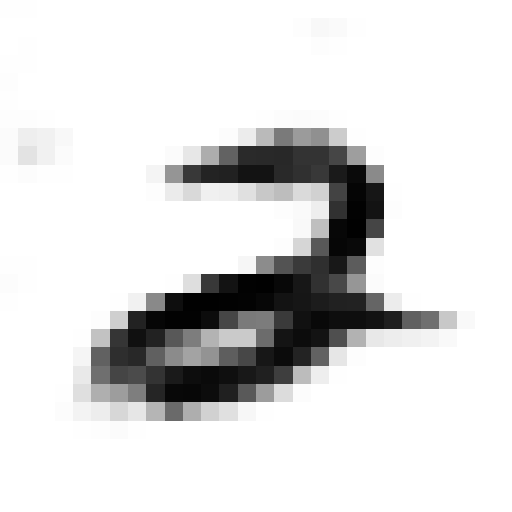
\includegraphics[width=30pt,height=30pt]{img/fake.png}};
%Image [id:dp6761500318437508] 
\draw (280,140) node  {
\includegraphics[width=30pt,height=30pt]{img/real.png}};
%Shape: Trapezoid [id:dp3595752922993056] 
\draw   (230,120) -- (130,144) -- (130,176) -- (230,200) -- cycle ;
%Shape: Trapezoid [id:dp017629486646709824] 
\draw   (330,200) -- (430,176) -- (430,144) -- (330,120) -- cycle ;
%Shape: Square [id:dp17681187394815812] 
\draw   (260,120) -- (300,120) -- (300,160) -- (260,160) -- cycle ;
%Shape: Square [id:dp9484762525415644] 
\draw   (260,160) -- (300,160) -- (300,200) -- (260,200) -- cycle ;

% Text Node
\draw (165,152.4) node [anchor=north west][inner sep=0.75pt]    {$G(\mathbf{z})$};
% Text Node
\draw (364,152.4) node [anchor=north west][inner sep=0.75pt]    {$D(\mathbf{x})$};
% Text Node
\draw (30,152.4) node [anchor=north west][inner sep=0.75pt]    {$\mathbf{z} \sim \mathcal{N}(\mathbf{0} ,\ \boldsymbol{\Sigma })$};
% Text Node
\draw (247,212.4) node [anchor=north west][inner sep=0.75pt]    {$\mathbf{x} \sim p_{g}(\mathbf{x})$};
% Text Node
\draw (238,90.4) node [anchor=north west][inner sep=0.75pt]    {$\mathbf{x} \sim p_{data}(\mathbf{x})$};
% Text Node
\draw (438,152.4) node [anchor=north west][inner sep=0.75pt]    {$real/fake$};
\end{tikzpicture}
\caption{A GAN trains a generator network $G$ to fool a discriminator network $D$ in emitting counterfeit images $\mathbf{x}$ by transforming noise input $\mathbf{z}$. In order to do so, $G$ must (implicitly) learn the data-generating distribution, $p_{data}$.}
\label{fig:gan_schematic}
\end{figure}

The GAN framework (Figure \ref{fig:gan_schematic}) is \emph{adversarial} in that it pits a pair of neural networks in a two-player minimax \emph{game}: a \emph{generator},

\begin{equation}
G : Z \to X,
\end{equation}

where in the simplest case $\mathbf{z} \sim Z$ is a vector of (uniform or Gaussian) noise and $\mathbf{x} \sim X$ is a synthetic data point (in particular, an image); and a \emph{discriminator},

\begin{equation}
D : X \to \{0, 1\},
\end{equation}

that is, a mapping from data point to binary value. $D$ aims to minimise its rate of failure in discerning true data from ``fake'' data sampled from the the generator, which aims to maximise the error made by the discriminator,

\begin{equation}
\max_G\min_D\mathcal{L}_{GAN}(D, G) = \mathbb{E}_{\mathbf{x} \sim p(\mathbf{x})}[\log D(\mathbf{x})] + \mathbb{E}_{\mathbf{z} \sim p(\mathbf{z})}[\log(1 - D(G(\mathbf{z})))]
\label{eq:gan_objective}
\end{equation}

The stationary point of Equation \ref{eq:gan_objective} is a \emph{Nash equilibrium} (a saddle point) between the two objectives. \cite{goodfellow2014generative} guarantee that the distribution implicitly defined\footnote{GANs are implicit generative models, in contrast to explicit models such as VAEs, which model the probabilities directly. GANs serve as an sample-emitting oracle emulating the true distribution.} by $G$, $p_g = p_{\text{data}}$ for $G^*$ at (global) optimality, and 

\begin{equation}
D^*(\mathbf{x}) = \frac{p_{\text{data}}(\mathbf{x})}{p_{\text{data}}(\mathbf{x}) + p_{g}(\mathbf{x})},
\end{equation}

where $p_{\text{data}}$ is the data-generating distribution. In practice, GANs are trained by backpropagation with alternating gradient descent between $D$ and $G$. The weights of $D$ are frozen while propagating the errors back through $D$ to $G$.

GAN architecture design must strike a balance between a generator expressive enough to approximate the data distribution, and a discriminator powerful enough to hold it to the task. GANs are chronically afflicted with a phenomenon known as \emph{mode collapse}. Mode collapse is the condition in which the generator ``collapses'' to generating few or even a unique output, regardless of the noise input $\mathbf{z}$. \cite{metz2016unrolled} differentiate two varieties of mode collapse: \emph{discrete mode collapse}, where the generator collapses to a subset of data modes (easily detected); and the more insidious \emph{manifold collapse}, where the generator collapses to a subspace of the data distribution. They reason that mode collapse originates from the fact that in each iteration of training, the generator is impelled towards a delta function at the mode considered most ``real'' by the discriminator. The discriminator responds by lowering the probability of this mode, leading to oscillations in generation. The ``unrolled'' GAN training approach that they advocate mitigates this tendency by informing the generator in advance of the discriminator's response to its prospective weight updates.

Another promising attempt to attenuate the mode collapse problem is to replace the Jensen-Shannon divergence loss function with the Earth Mover (EM) or Wasserstein-1 distance. Such is the strategy of Wasserstein GANs (WGANs). Intuitively, the EM distance measures a distance between two distributions. We can write the EM distance as the quantity $\mathbb{E}_{x \sim \mathbb{P}_r}[f_w(x)] - \mathbb{E}_{z\sim p(z)}[f_w(g_{\theta}(z))]$ maximised by choice of $f_w$ (discriminator). The goal is then to minimise this distance through optimisation of the generator. The training algorithm is very similar to GANs. WGANs are more stable, as the substituted loss function allows the discriminator to be trained to optimality. This greatly mitigates the mode collapse problem. Nevertheless, more subtle forms of partial mode collapse remain a recurrent problem for GANs. As a bonus, the discriminator loss (estimated EM distance) becomes meaningful during training, interpretable as image sample quality, rendering the implementation and fine-tuning of WGANs far easier. Despite the merits of WGANs, we do not have recourse to them in this dissertation.

\subsection{Deep convolutional GANs}

\cite{radford2015unsupervised} first succeeded in training more powerful, high-resolution GANs, by identifying a set of design principles: replacing pooling layers with strided convolutions; removing fully-connected layers (apart from the first layer of the generator); using batch normalisation after all but the last layer; using a $\tanh$ activation at the end of the generator (and ReLU everywhere else); and using LeakyReLU activations everywhere in the discriminator. Deep convolutional GANs (DC-GANs) represent a vast improvement over the original fully-connected GANs.

\subsection{Conditional GANs}

\cite{mirza2014conditional} present a simple extension to GANs allowing for control over the data generating process. One simply includes an additional input $\mathbf{y} \sim Y$ (for example, class information), to obtain conditional GANs (cGANs). That is, now the generator is conditional,

\begin{equation}
G : Z, Y \to X,
\end{equation}

as is the discriminator,

\begin{equation}
G : X, Y \to \{0, 1\},
\end{equation}

and the cGAN is trained against the objective,

\begin{align}\mathcal{L}_{cGAN}(D, G) = \mathbb{E}_{\mathbf{x} \sim p(\mathbf{x})}[\log D(\mathbf{x} | \mathbf{y})] + \mathbb{E}_{\mathbf{z} \sim p(\mathbf{z})}[\log(1 - D(G(\mathbf{z} | \mathbf{y})))]
\end{align}

\cite{mirza2014conditional} does not offer so much as an intuition as to why conditional GANs works (seemingly the article was written in a hurry), but it can be instructive to consider. As $D$ learns to associate conditional information such as object class with the ground truth images, it will declare ``fake'' any image emitted by $G$ not conforming to the condition, no matter the quality of the image. If $G$ is to succeed, it will be forced to generate images in adherence to the condition. The outcome of successful training is therefore a generator that can, for example, synthesise an authentic-looking image of a desired class on demand.

The implementation of cGANs is a straightforward modification to GANs: the conditional information is concatenated to the typical usual inputs of both $D$ and $G$ and fed to further hidden layers. A DCGAN discriminator may, however, concatenate the conditional information after its convolutional layers.

\subsection{Assorted GANs}

The success of GANs have led to many interesting results in recent years. Image-to-image translation has been achieved with \texttt{pix2pix} (\cite{isola2017image}), a GAN conditioned on a full image serving as a blueprint for the generated image. Such models are capable of an endless variety of applications, including segmentation and image colourisation. CycleGANs (\cite{zhu2017unpaired}) achieve \emph{unpaired} image-to-image translation, learning to map between image domains in an unsupervised way. Application include style transfer. RecycleGANs (\cite{bansal2018recycle}) achieve the same for video-to-video retargeting.

Elsewhere, progressive growing of GANs (\cite{karras2017progressive}) produce high resolution outputs (up to $1024\times1024$ pixels). Here, training is done in stages, beginning at low resolutions ($4\times4$), and doubling the resolution at intervals. This is done simply by adding new layers to the generator and discriminator, which remain symmetric throughout training. Thus, the GAN learns global structures first at low resolution, progressively refining its output.

